\documentclass[journal]{IEEEtran}
%\usepackage[autostyle]{csquotes}
\usepackage{graphicx}
\usepackage{soul}
\usepackage{float}
\usepackage{multirow}
\usepackage{booktabs}
\usepackage{amssymb}
\usepackage{amsmath}
\usepackage{longtable}
\usepackage{subfig}
\usepackage{multirow}
\usepackage{csquotes}
\usepackage[T1]{fontenc}
\usepackage[table]{xcolor}
\usepackage[pagebackref=true,breaklinks=true,colorlinks,bookmarks=false]{hyperref}

\hyphenation{op-tical net-works semi-conduc-tor}

\def\SA#1{{\color{red}{\bf [Saeed:} {\it{#1}}{\bf ]}}}
\begin{document}
\title{A Comprehensive Overview of Large Language Models}

\author{\IEEEauthorblockN{Humza Naveed, Asad Ullah Khan*, Shi Qiu*, Muhammad Saqib*, \\Saeed Anwar, Muhammad Usman, Nick Barnes, Ajmal Mian}% <-this % stops a space
\IEEEcompsocitemizethanks{
\IEEEcompsocthanksitem Version: 01 (update on July 10, 2023).  
\IEEEcompsocthanksitem GitHub link: \url{https://github.com/humza909/LLM_Survey.git} 
\IEEEcompsocthanksitem * is for equal contribution. 
\IEEEcompsocthanksitem 
Contact e-mail: humza\_naveed@yahoo.com}}


%\thanks{M. Shell was with the Department
%of Electrical and Computer Engineering, Georgia Institute of Technology, Atlanta,
%GA, 30332 USA e-mail: (see http://www.michaelshell.org/contact.html).}% <-this % stops a space
%\thanks{J. Doe and J. Doe are with Anonymous University.}% <-this % stops a space
%\thanks{Manuscript received 19 April 2005; revised 26 August 2015.}}

\markboth{Journal of \LaTeX\ }%
{Shell \MakeLowercase{\textit{et al.}}: Bare Demo of IEEEtran.cls for IEEE Journals}

\maketitle
\begin{abstract}
% Large Language Models (LLMs) have shown excellent generalization abilities that lead to the development of numerous models. These models suggest different approaches, for example, increasing model parameters, training data, tweaking architecture, training strategies, and pipelines to outperform baselines. Analyzing these aspects is important to identify changes that bring stability to the training and better generalization for the LLMs. In this paper, we summarize these fine-grained details of LLMs. Initially, we provide a background for the LLMs to discuss basic building blocks followed by a comprehensive overview of LLMs. The end of the paper discusses important findings by the LLMs and summarizes important architectural and training strategies to develop better LLMs. Because of the continuous development in LLMs, we will update this paper regularly with new sections and LLMs.  

Large Language Models (LLMs) have shown excellent generalization capabilities that have led to the development of numerous models. These models propose various new architectures, tweaking existing architectures with refined training strategies, increasing context length, using high-quality training data, and increasing training time to outperform baselines. Analyzing new developments is crucial for identifying changes that enhance training stability and improve generalization in LLMs. This survey paper comprehensively analyses the LLMs architectures and their categorization, training strategies, training datasets, and performance evaluations and discusses future research directions. Moreover, the paper also discusses the basic building blocks and concepts behind LLMs, followed by a complete overview of LLMs, including their important features and functions. Finally, the paper summarizes significant findings from LLM research and consolidates essential architectural and training strategies for developing advanced LLMs. Given the continuous advancements in LLMs, we intend to regularly update this paper by incorporating new sections and featuring the latest LLM models.
\end{abstract}
\begin{IEEEkeywords}
Large Language Models, LLMs, auto-regressive models, encoder-decoder, training pipeline, architecture, survey, review
\end{IEEEkeywords}

\IEEEpeerreviewmaketitle
\section{Introduction}

Language plays a fundamental role in facilitating communication and self-expression for humans, and likewise, communication holds paramount importance for machines in their interactions with humans and other systems. Large Language Models (LLMs) have emerged as cutting-edge artificial intelligence systems designed to process and generate text, aiming to communicate coherently~\cite{y2022large}. The need for LLMs stems from the growing demand for machines to handle complex language tasks, including translation, summarization, information retrieval, and conversational interactions. 
Recently, significant breakthroughs have been witnessed in language models, primarily attributed to deep learning techniques, advancements in neural architectures like transformers, increased computational capabilities, and the accessibility of training data extracted from the internet~\cite{chernyavskiy2021transformers}. These developments have brought about a revolutionary transformation by enabling the creation of Large Language Models (LLMs) that can approximate human-level performance on certain evaluation benchmarks~\cite{wang2019superglue,adiwardana2020towards}. 


\begin{figure}[tbp]
\centering
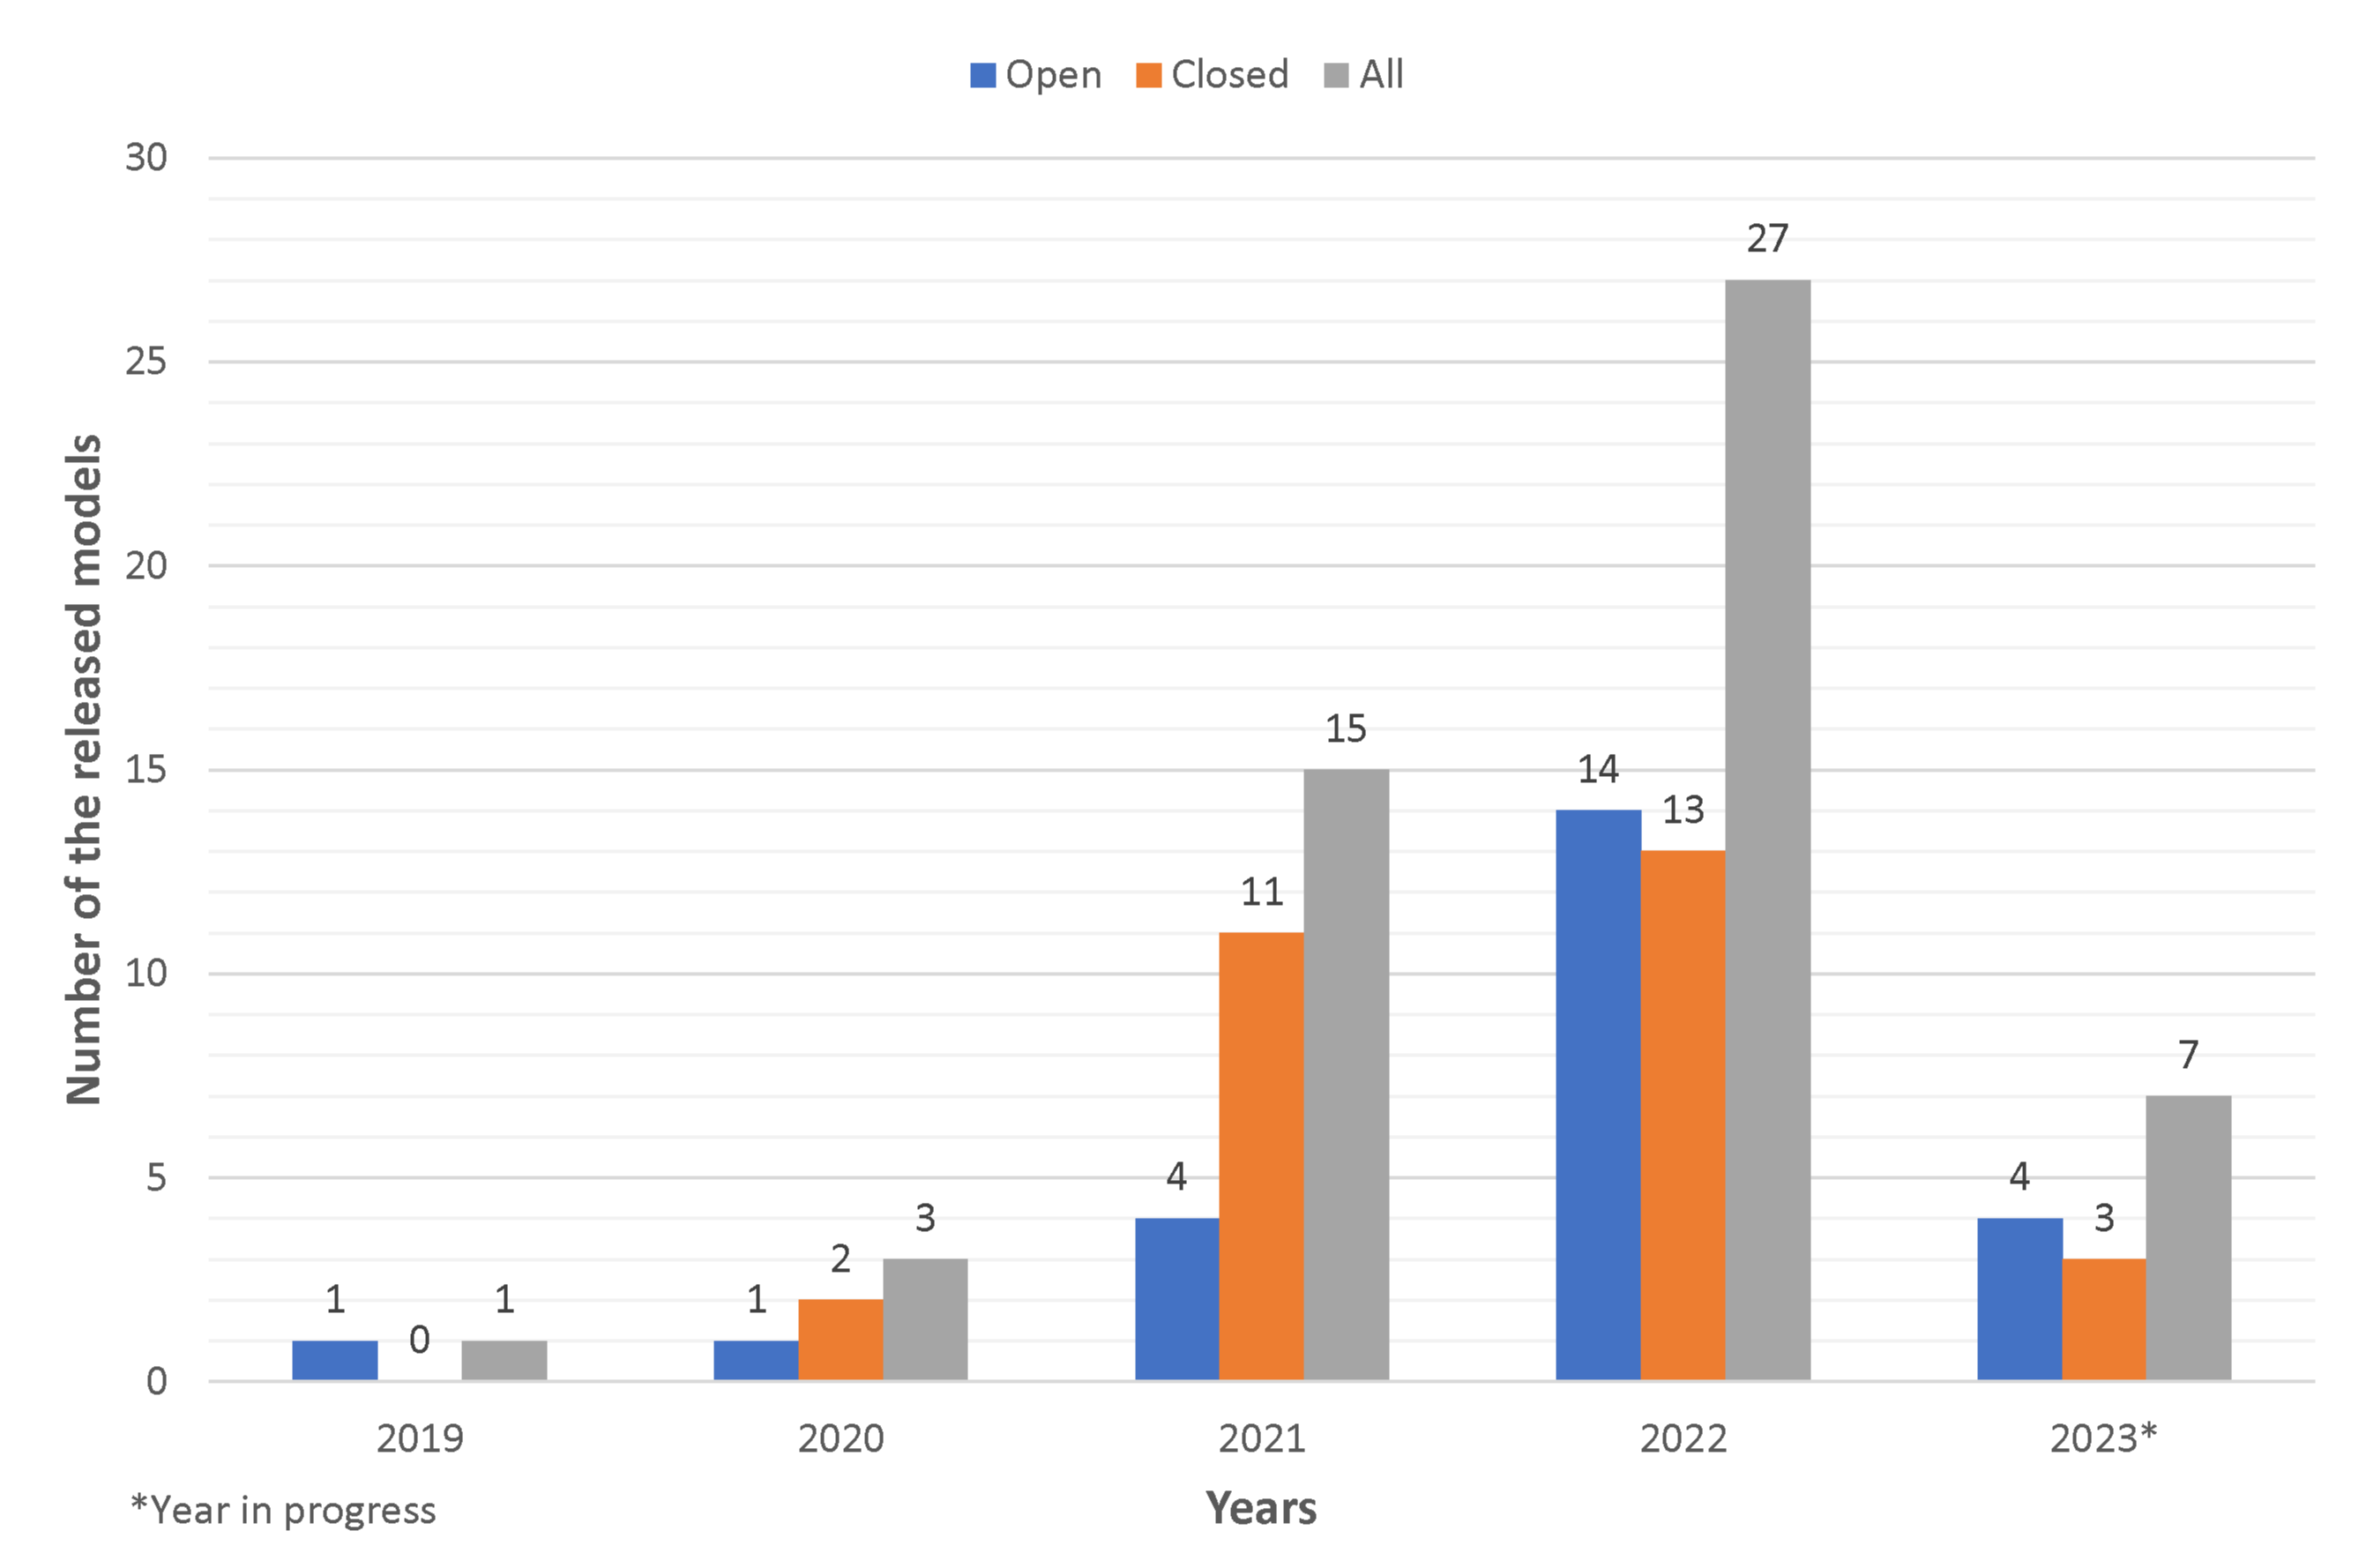
\includegraphics[width=1\columnwidth]{Figure/Column_Chart.png}
\caption{The trends in the number of LLM models introduced over the years.}
%\caption{Number of LLMs introduced over the years.}
\label{fig:num_LLMs_barchart}
\end{figure}

\begin{figure*}[tbp]
\centering
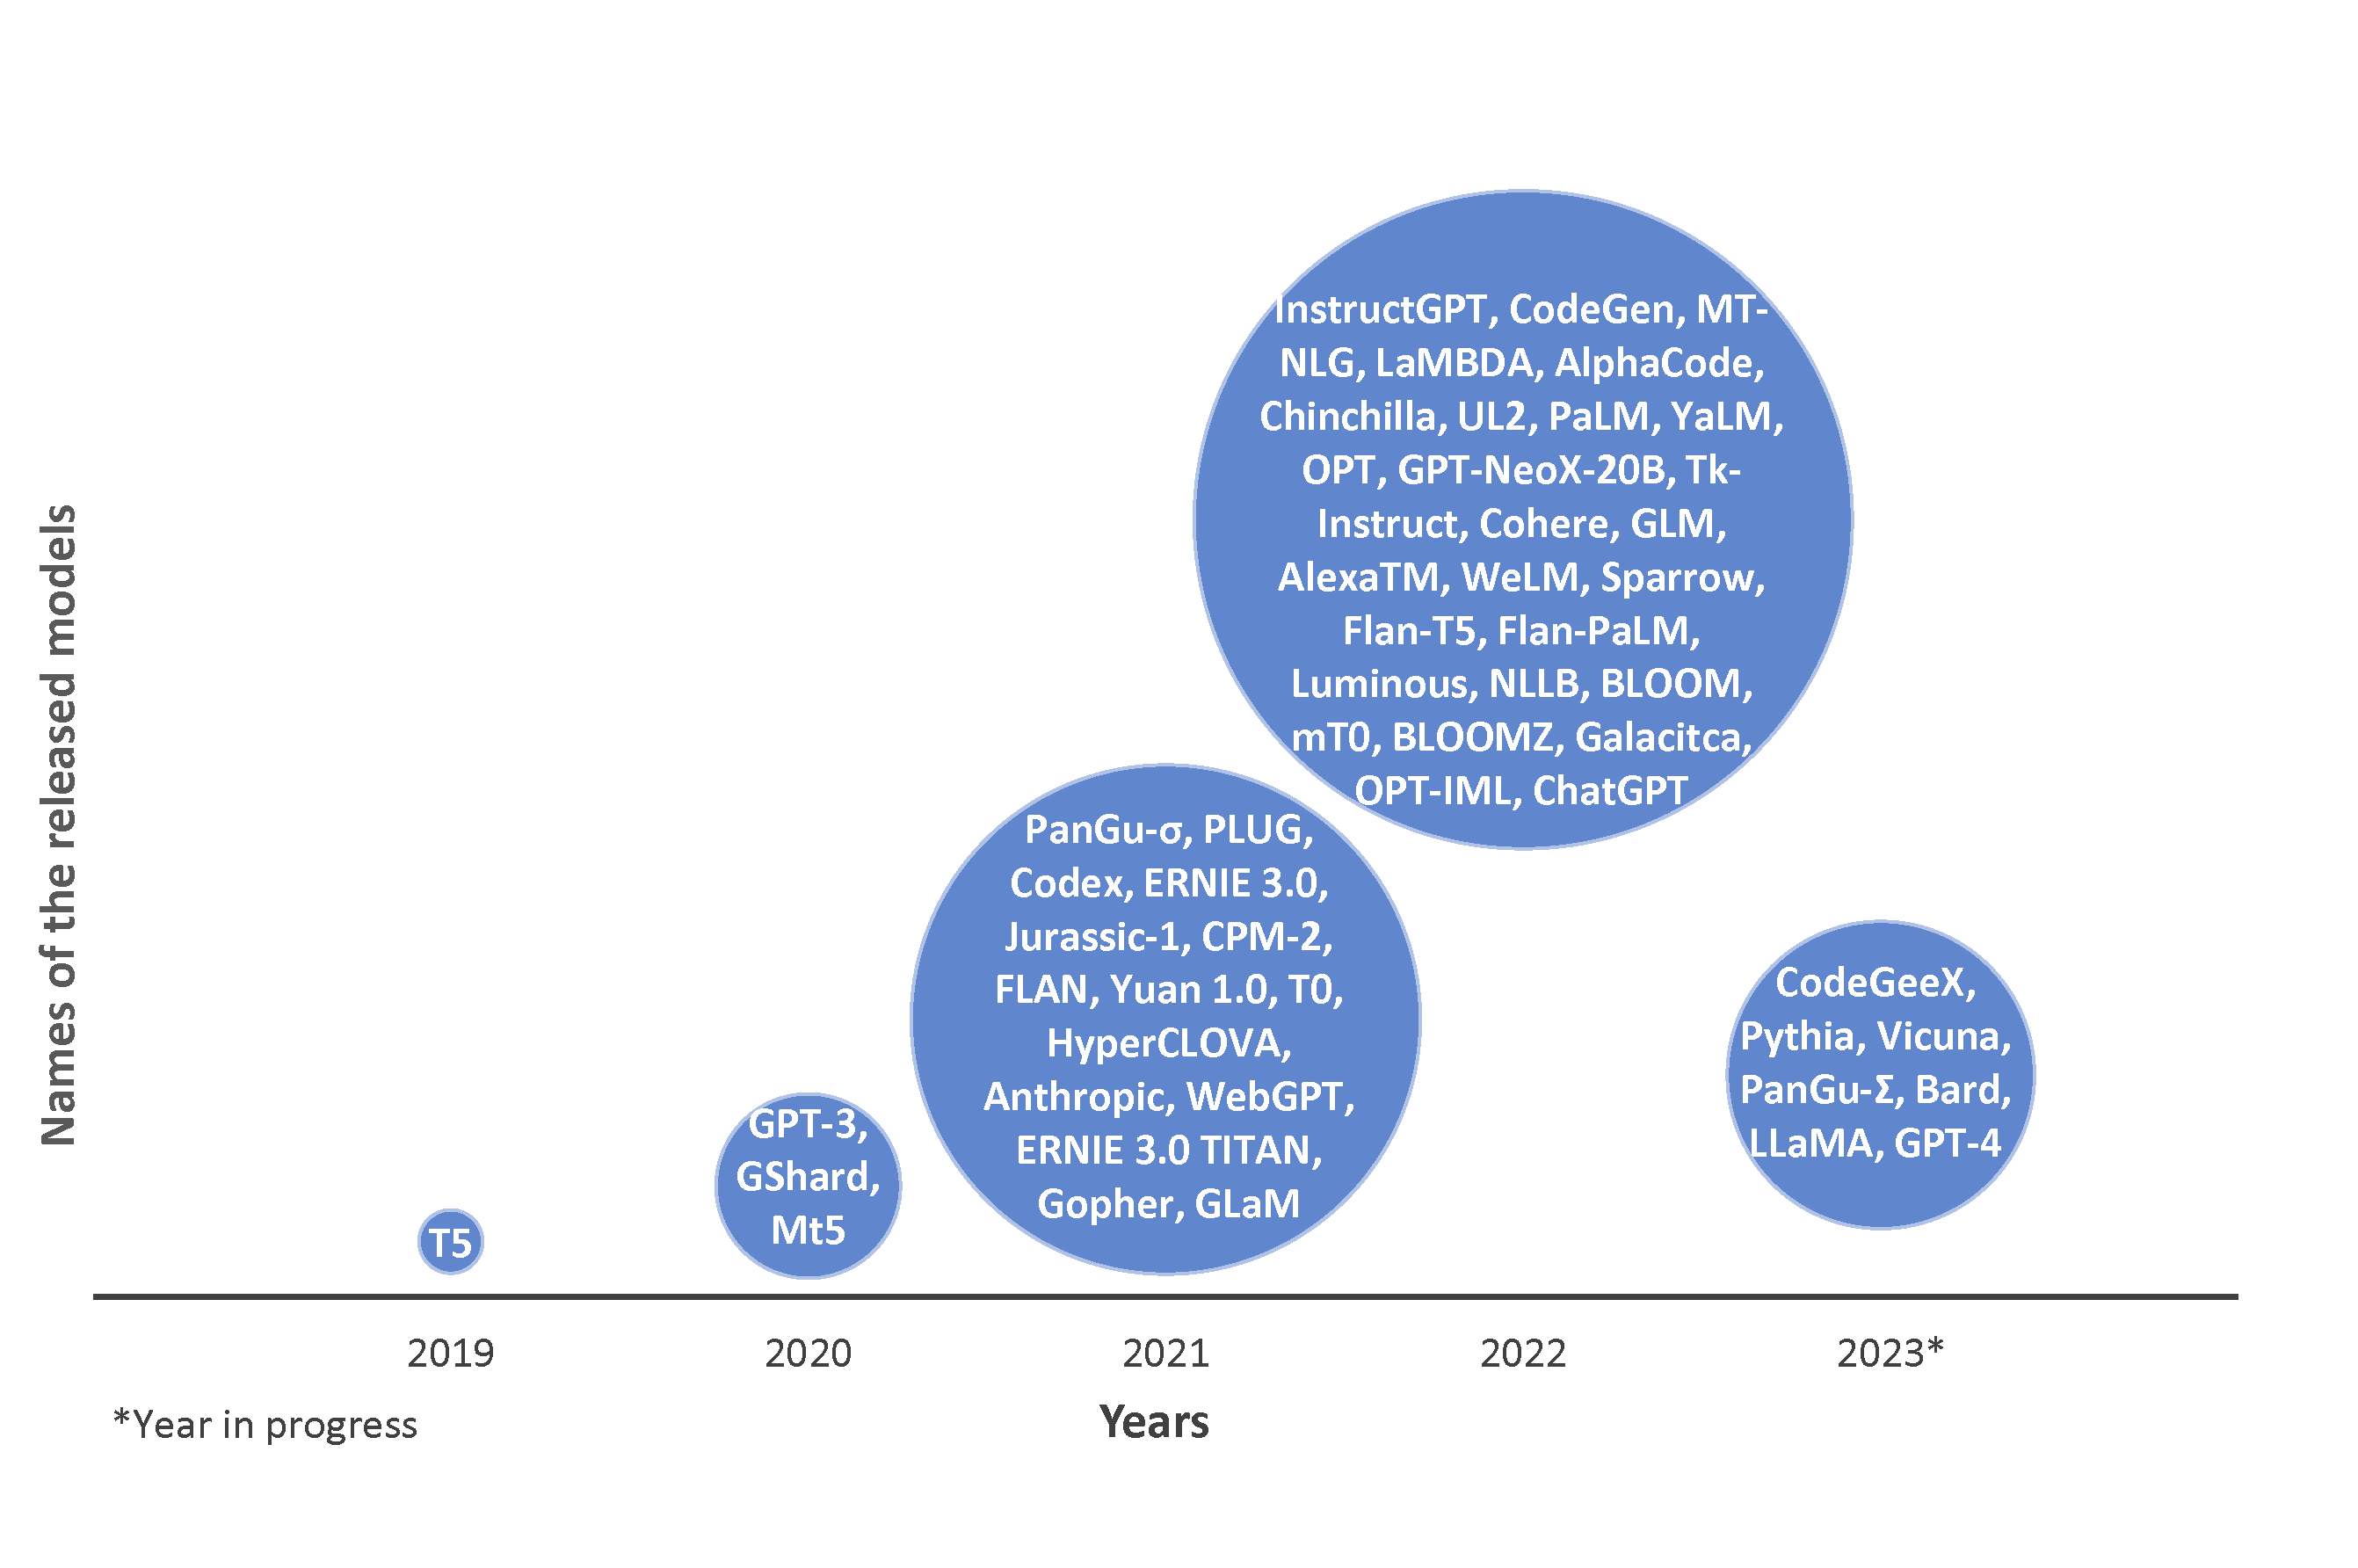
\includegraphics[width=2\columnwidth]{Figure/Bubble_Chart.png}
\caption{The progressive introduction of LLM models demonstrates advances in natural language processing explicitly adapted to various fields and provides increased research,  analysis, and application capabilities.}
%\caption{LLMs introduced over the years.}
\label{fig:LLMs_bubblechart}
\end{figure*}

LLMs, particularly pre-trained language models (PLM), have shown tremendous generalization abilities for text understanding and generation tasks while trained in a self-supervised setting on a large corpus of text~\cite{Bert, ELMO, BART}. The performance of pre-trained language models (PLMs) improves significantly when fine-tuned for downstream tasks, surpassing the performance of models trained from scratch. These characteristics of language models motivated researchers to train larger PLMs on even bigger datasets and found that scaling model and dataset size further improve the generalization abilities. 

Now modern LLMs are capable of performing various tasks like code generation, text generation, tool manipulation, reasoning, and understanding in zero-shot and few-shot settings in diverse domains, even without requiring any fine-tuning on downstream tasks~\cite{GPT-3, BLOOM, OPT}. Such generalization was previously unattainable with smaller models, marking a significant advancement in language modeling. This development has sparked enthusiasm and excitement within the research community for the enhancement of LLM architectures and training strategies, leading to the development of numerous LLMs~\cite{T5, mT5, CPM-2, GPT-3, BLOOM, OPT, PaLM}. 

% The graph~\ref{fig:num_LLMs_barchart} illustrates a growing trend in the number of released LLMs, including open-source and closed-source models, over the years.

The graph presented in Fig~\ref{fig:num_LLMs_barchart} depicts an increasing trend in the number of released LLMs, including open-source and closed-source models, over the years. Furthermore, Fig~\ref{fig:LLMs_bubblechart} highlights the names of significant releases of various LLMs.



% In recent years, pre-trained language models (PLM) have shown tremendous generalization abilities for text understanding and generation tasks while being trained in a self-supervised setting on a large corpus~\cite{Bert, ELMO, BART}. PLMs perform better when fine-tuned for downstream tasks as compared to the models trained from scratch. These characteristics of language models motivated researchers to train larger PLMs on even bigger datasets and found scaling model and dataset size further improve the generalization abilities. These huge models are given the name Large Language Models (LLMs).  \\
% LLMs are capable to perform diverse tasks like code generation, text generation, tool manipulation, reasoning, and understanding in zero-shot and few-shot settings in diverse domains, without requiring any fine-tuning on downstream tasks~\cite{GPT-3, BLOOM, OPT}. Such a generalized capacity was not possible with smaller models. This created a spark in the research community to propose better LLMs architectures and training strategies leading to the development of numerous LLMs~\cite{T5, mT5, CPM-2, GPT-3, BLOOM, OPT, PaLM}.   \\




During the early days of Large Language Models (LLMs), many research efforts focused on developing models for transfer learning to downstream tasks ~\cite{T5, mT5, UL2} until the emergence of models like GPT-3~\cite{GPT-3}, which demonstrated impressive performance even without fine-tuning. Due to the closed-source nature of GPT-3, there was a demand for open-source alternatives, leading to the development of various models ~\cite{BLOOM, OPT} operating at the scale of GPT-3 and trained on extensive web-based datasets~\cite{Common_Crawl,Wikipedia,Openwebtext_Dataset,BQ_Dataset}.   Subsequently, researchers proposed several architectural designs and training strategies that showed superior performance compared to GPT-3 across various tasks ~\cite{UL2, PaLM, U-PaLM, mtnlg}. 

The performance of LLMs improves further with instruction fine-tuning, outperforming pre-trained LLMs on various benchmarks~\cite{T0, mT0andBLOOMZ}. Instruction fine-tuning of LLMs refers to a specific training approach by incorporating additional prompts or instructions during the fine-tuning phase to guide the output and thus enable the users to have more fine-grained control over the outputs of LLMs. These prompts can be natural language instructions or example demonstrations based on the task's requirement. In the literature, different datasets have been curated for instruction fine-tuning. These datasets include more instances and tasks that further improve the performance over baselines~\cite{OPT_IML,mT0andBLOOMZ,Flan,Tk-INSTRUCT}. When performing instruction fine-tuning, all the model parameters need to be updated. However, parameter-efficient fine-tuning takes a different approach by updating only a small number of parameters while still maintaining good performance. This method keeps the original model frozen and adds a few extra parameters at different locations within the model~\cite{LMAdapted, LMAdapter_2, LMAdapter_3, Prompt_Tuning, Prefix_Tuning}. This approach helps achieve efficient fine-tuning while minimizing the impact on the model's overall performance.
% Instruction-tuning requires updating all the parameters. Compared to this, parameter-efficient fine-tuning updates only a small number of parameters without dropping the performance significantly. In this method, the original model is kept frozen and fewer additional parameters are added to the model at different positions as given in~\cite{LMAdapted, LMAdapter_2, LMAdapter_3, Prompt_Tuning, Prefix_Tuning}.  



The literature presents numerous pre-trained and fine-tuned models for LLMs with diverse approaches. Some survey papers provide an overview of augmented techniques in LLMs~\cite{survey_1}. Additionally, a comprehensive review is available that covers architectures, fine-tuning, emergent abilities, and the usability of LLMs~\cite{Survey_LLM}. Another survey provides a historical account of foundation models~\cite{survey_2}. However, these review papers do not delve into the specific details of individual models, offering only a surface-level understanding of architectures and training methods. In contrast, our paper aims to provide a more in-depth analysis of individual LLMs by discussing fine-grained details.


The absence of comprehensive and detailed discussions, particularly from a historical standpoint, regarding the architecture, training datasets, and other granular aspects of Large Language Models (LLMs), has motivated us to undertake an exhaustive survey. This survey aims to provide an in-depth and comprehensive analysis of LLMs, delving into the details surrounding their development, architecture, training datasets, and related components.
\begin{itemize}
\item To the best of our knowledge, this is the first comprehensive survey paper that discusses fine-grained details of LLMs. 
%Write about our survey and the contributions etc
\item We provide a thorough analysis of the existing literature regarding various LLMs architectures
and their categorization. Moreover, we also discussed the basics of the LLMs to make the paper self-sufficient and productive for the reader not familiar with LLMs.

% \item We have also identified future research directions that might help researchers to further enhance the methods and achieve new state-of-the-art.



\item Our paper focuses on providing comprehensive details for each LLM model and covers aspects such as architecture modifications, training objectives, datasets used, strategies for stable training, key findings, suggestions, and challenges encountered during training.

\item We aim to summarize these crucial details in our paper to assist researchers in identifying better architectures and training approaches for their work.
\end{itemize}


% Our paper focuses on providing comprehensive details for each LLM model and covers aspects such as architecture modifications, training objectives, datasets used, strategies for stable training, key findings, suggestions, and challenges encountered during training.
Our paper complements a recent survey paper~\cite{Survey_LLM} on LLMs that covers topics like data preprocessing, data cleaning, scaling laws, emergent abilities, adaptation tuning, and utilization. While the survey paper provides information on architectures, it does not delve into the fine-grained details of architectural changes, training objectives, and specific findings from proposed LLMs. 
% For every LLM, we provide details on changes in architecture, training objective, datasets, and strategies to stable training, findings and suggestions by every LLM, and other issues faced during training. Our paper complements a recent survey paper on LLMs that explains various topics on data preprocessing, data cleaning, scaling laws, emergent abilities, adaptation tuning, and utilization. It also provides information on architectures but does not discuss fine details on architectural changes, training objectives and findings of proposed LLMs. We summarize these details in this paper with the aim to help researchers in identifying better architectures and training approaches in their research work.    \\
We discuss LLMs model with a minimum of 10 billion parameters or more similar to the paper~\cite{Survey_LLM}. Models smaller than this scale are not discussed in our paper. One can refer to review papers such as~\cite{survey_smaller_LLMs_1, survey_smaller_LLMs_2, survey_1} for exploring smaller models.


% Similar to the paper~\cite{Survey_LLM}, our definition of LLM is a model with at-least 10B or more parameters. We do not discuss models smaller than the 10B scale. One can see a review of these smaller models in~\cite{survey_smaller_LLMs_1, survey_smaller_LLMs_2, survey_1}. \\
     

The organization of this paper is as follows. Section~\ref{sec:Background} discusses the background of LLMs, offering a concise overview of the essential building blocks that constitute these models. We discuss architectural styles, fine-tuning strategies, libraries, and distributed training methods. This section serves as a foundation for understanding the subsequent discussions on LLMs. Section~\ref{sec_review} focuses on LLMs overview, architectures, and training pipelines and strategies. Section~\ref{sec:Findings} presents the key findings derived from each LLM. Section~\ref{Model_Configurations_} highlights the configuration and parameters that play a crucial role in the functioning of these models. The LLM training and evaluation benchmarks are discussed in section~\ref{Datasets_and_Evaluation_}, followed by concluding remarks and future direction in the conclusion section.
\section{Background}
\label{sec:Background}
\subsection{Tokenization}
\label{ss:tokenization}
LLMs are trained on text to predict text, and similar to other natural language processing systems, they use tokenization~\cite{webster1992tokenization} as the essential preprocessing step. It aims to parse the text into non-decomposing units called tokens. Tokens can be characters, subwords~\cite{unigramLM}, symbols~\cite{bpe}, or words, depending on the size and type of the model. Some of the commonly used tokenization schemes in LLMs are briefed here. Readers are encouraged to refer to~\cite{tokenizationsurvey} for a detailed survey.

\subsubsection{WordPiece~\cite{wordpiece}}
\label{ss:wordpiece}
It was introduced in~\cite{wordpiece} as a novel text segmentation technique for Japanese and Korean languages to improve the language model for voice search systems. WordPiece selects tokens that increase the likelihood of an n-gram-based language model trained on the vocabulary composed of tokens.

\subsubsection{BPE~\cite{bpe}}
\label{ss:bpe}
Byte Pair Encoding (BPE) has its origin in compression algorithms. It is an iterative process of generating tokens where pairs of adjacent \textit{symbols} are replaced by a new symbol, and the occurrences of the most occurring symbols in the input text are merged together.

\subsubsection{UnigramLM~\cite{unigramLM}}
\label{ss:unigramLM}
In this tokenization, a simple unigram language model (LM) is trained using an initial vocabulary of \textit{subword} units. The vocabulary is pruned iteratively by removing the lowest-probability items from the list, which are the worst performing on the unigram LM.

\subsection{Attention}
\label{ss:attention}
Attention, particularly \textit{selective attention}, has been widely studied under perception, psychophysics and psychology. Selective attention can be conceived as \enquote{the programming by the O of which stimuli will be processed or encoded and in what order this will occur}~\cite{selectiveattention}. While this definition has its roots in visual perception, it has uncanny similarities with the recently formulated \textit{attention}~\cite{attention, Transformers} (which stimuli will be processed) and \textit{positional encoding} (in what order this will occur)~\cite{Transformers} in LLMs. We discuss both in sections~\ref{ss:llmattention} and~\ref{ss:encodingposition}, respectively. 

\subsection{Attention in LLMs}
\label{ss:llmattention}
The attention mechanism computes a representation of the input sequences by relating different positions (\textit{tokens}) of these sequences. There are various approaches to calculating and implementing attention, out of which some famous types are given below.

\subsubsection{Self-Attention~\cite{Transformers}}
\label{ss:selfattention}
The self-attention is also known as intra-attention since all the queries, keys and values come from the same block (encoder or decoder). The self-attention layer connects all the sequence positions to each other with $O(1)$ space complexity which is highly desirable for learning long-range dependencies in the input. 

\subsubsection{Cross Attention}
\label{ss:crossattention}
In encoder-decoder architectures, the outputs of the encoder blocks act as the queries to the intermediate representation of the decoder, which provides the keys and values to calculate a representation of the decoder conditioned on the encoder. This attention is called cross-attention.

\subsubsection{Full Attention}
\label{ss:fullattention}
The naive implementation of calculating self-attention is known as full attention.

\subsubsection{Sparse Attention~\cite{sparse_transformer}}
\label{ss:sparseattention}
The self-attention has a time complexity of $O(n^2)$, which becomes prohibitive when scaling the LLMs to large context windows. An approximation to the self-attention was proposed in~\cite{sparse_transformer}, which greatly enhanced the capacity of GPT series LLMs to process a greater number of input tokens in a reasonable time.

\subsubsection{Flash Attention~\cite{flashattention}}
\label{ss:flashattention}
The bottleneck for calculating the attention using GPUs lies in the memory access rather than the computational speed. Flash Attention uses the classical input tiling approach in order to process the blocks of the input in GPU on-chip SRAM rather than doing IO for every token from the High Bandwith Memory (HBM). An extension of this approach to sparse attention follows the speed gains of the full attention implementation. This trick allows even greater context-length windows in the LLMs as compared to those LLMs with sparse attention.

\subsection{Encoding Positions}
\label{ss:encodingposition}
The \textit{attention} modules do not consider the order of processing by design. Transformer~\cite{Transformers} introduced \enquote{positional encodings} to feed information about the position of the tokens in input sequences. Several variants of positional encoding have been proposed~\cite{alibi, su2021roformer}. Interestingly, a recent study~\cite{NoPE} suggests that adding this information may not matter for the state-of-the-art decoder-only Transformers.

\subsubsection{Absolute}
This is the most straightforward approach to adding the sequence order information by assigning a unique identifier to each position of the sequence before passing it to the attention module.

\subsubsection{Relative}
In order to pass the information of the relative dependencies of different tokens appearing at different locations in the sequence, a relative positional encoding is calculated by some kind of learning. Two famous types of relative encodings are: 

\noindent
\emph{\textbf{Alibi}~\cite{alibi}} In this approach, a scalar bias is subtracted from the attention score calculated using two tokens which increases with the distance between the positions of the tokens. This learned approach effectively favors using recent tokens for attention. 

\noindent
\emph{\textbf{RoPE}} Keys, queries and values are all vectors in the LLMs. RoPE~\cite{su2021roformer} involves the rotation of the query and key representations at an angle proportional to their absolute positions of the tokens in the input sequence. This step results in a relative positional encoding scheme which decays with the distance between the tokens.

\subsection{Activation Functions}
\label{sec:activation functions}
The activation functions serve a crucial role in the curve-fitting abilities of the neural networks, as proved in~\cite{activationfunction}. The modern activation functions used in LLMs are different from the earlier squashing functions but are critical to the success of LLMs. We discuss these activation functions in this section.  

\subsubsection{ReLU~\cite{relu}}
\label{ss:relu}
Rectified linear unit (ReLU) is defined as
\begin{equation}
ReLU(x) = max(0,x)    
\label{eq:relu}
\end{equation}

\subsubsection{GeLU~\cite{gelu}}
\label{ss:gelu}
Gaussian Error Linear Unit (GeLU) is the combination of ReLU,  dropout~\cite{srivastava2014dropout} and zoneout~\cite{krueger2016zoneout}. It is the most widely used activation function in contemporary LLM literature.

\subsubsection{GLU variants~\cite{shazeer2020glu}}
\label{ss:gluvariants}
Gated Linear Unit~\cite{glu} is a neural network layer that is an element-wise product ($\otimes$) of a linear transformation and a sigmoid transformed ($\sigma$) linear projection of the input given as
\begin{equation}
GLU(x, W, V, b, c) = (xW + b) \otimes \sigma (xV + c),
\end{equation}
where $X$ is the input of layer and $l$, $W, b, V \textnormal{ and }c$ are learned parameters.

GLU was modified in~\cite{shazeer2020glu} to evaluate the effect of different variations in the training and testing of transformers, resulting in better empirical results. Here are the different GLU variations introduced in~\cite{shazeer2020glu} and used in LLMs. 

\begin{align*}
ReGLU(x, W, V, b, c) &= max(0, xW + b) \otimes , \\
GEGLU(x, W, V, b, c) &= GELU(xW + b) \otimes (xV + c), \\
SwiGLU(x, W, V, b, c, \beta) &= Swish\beta (xW + b) \otimes (xV + c).          
\end{align*}

\subsection{Layer Normalization}
\label{sec:layernormalization}
Layer normalization leads to faster convergence and is a widely used component in transformers. In this section, we provide different normalization techniques widely used in LLM literature.

\subsubsection{LayerNorm}
\label{ss:layernorm}
Layer norm computes statistics over all the hidden units in a layer $(l)$ as follows: 
\begin{equation}
u^l = \frac{1}{n} \sum_{i}^{n} a_i^l \hspace{2em} \sigma^l = \sqrt{\frac{1}{n} \sum_{i}^{n} (a_i^l - u^l)^2} ,
\end{equation}
where $n$ is the number of neurons in the layer $l$ and $a_i^l$ is the summed input of the $i$ neuron in layer $l$. LayerNorm provides invariance to rescaling of the weights and re-centering of the distribution.

\subsubsection{RMSNorm}
~\cite{rmsnorm} proposed that the invariance properties of LayerNorm are spurious, and we can achieve the same performance benefits as we get from LayerNorm by using a computationally efficient normalization technique that trades off re-centering invariance with speed. LayerNorm gives the normalized summed input to layer $l$ as follows
\begin{equation}
\overline{a_i^l} = \frac{a_i^l - u^l}{\sigma}g_i^l 
\end{equation}
where $g_i^l$ is the gain parameter. RMSNorm~\cite{rmsnorm} modifies $\overline{a_i^l}$ as

\begin{equation}
\overline{a_i^l} = \frac{a_i^l}{\textnormal{RMS}(\mathbf{a}^l)} g_i^l, \hspace{0.3em} \textnormal{where} \hspace{0.3em} \textnormal{RMS}(\mathbf{a}^l) = \sqrt{\frac{1}{n}\sum_{i}^{n}(a_i^l)^2}.
\end{equation}

\subsubsection{Pre-Norm and Post-Norm}
LLMs use transformer~\cite{Transformers} architecture with some variations. The original implementation~\cite{Transformers} used layer normalization after the residual connection, commonly called post-LN, concerning the order of \textit{Multihead attention – Residual – LN}. There is another order of the normalization, referred to as pre-LN~\cite{preLN} due to the position of the normalization step before the self-attention layer as in \textit{LN – Multihead attention – Residual}. Pre-LN is known to provide more stability in the training~\cite{shleifer2021normformer}. 

\subsubsection{DeepNorm}
While pre-LN has certain benefits over post-LN training, pre-LN training has an unwanted effect on the gradients~\cite{shleifer2021normformer}. The earlier layers have larger gradients than those at the bottom. DeepNorm~\cite{deepnorm} mitigates these adverse effects on the gradients. It is given as
\begin{equation}
\mathbf{x}^{l_f} = LN(\alpha \mathbf{x}^{l_p} + G^{l_p}(\mathbf{x}^{l_p}, {\boldmath\theta}{^{l_p}}), 
\end{equation}
where $\alpha$ is a constant and $\theta^{l_p}$ represents the parameters of layer $l_p$. These parameters are scaled by another constant $\beta$. Both of these constants depend only on the architecture. 

\subsection{Distributed LLM Training}
This section describes distributed LLM training approaches briefly. A more detailed discussion is available in~\cite{Survey_LLM}. 

\subsubsection{Data Parallelism}
Data parallelism replicates the model on multiple devices where data in a batch gets divided across devices. At the end of each training iteration weights are synchronized across all devices.    

\subsubsection{Tensor Parallelism}
Tensor parallelism shards a tensor computation across devices. It is also known as horizontal parallelism or intra-layer model parallelism.

\subsubsection{Pipeline Parallelism}
Pipeline parallelism shards model layers across different devices. This is also known as vertical parallelism.

\subsubsection{Model Parallelism}
A combination of tensor and pipeline parallelism is known as model parallelism.
\subsubsection{3D Parallelism}
A combination of data, tensor, and model parallelism is known as 3D parallelism.

\subsubsection{Optimizer Parallelism}
Optimizer parallelism also known as zero redundancy optimizer~\cite{ZeroOpt} implements optimizer state partitioning, gradient partitioning, and parameter partitioning across devices to reduce memory consumption while keeping the communication costs as low as possible. 

\subsubsection{Rematerialization}

\subsection{Libraries}
Some commonly used libraries for LLM training are: 1) Transformer~\cite{Lib_Transformers}, 2) DeepSpeed~\cite{Lib_DeepSpeed}, 3) Megatraon-LM~\cite{Lib_Megatron}, 4) JAX~\cite{Lib_Jax}, 5) Colossal-AI~\cite{Lib_Colossal}, 6) BMTrain~\cite{Lib_Bmtrain}, 7) FastMoE~\cite{Lib_Fastmoe}, and frameworks are 1) MindSpore~\cite{Lib_Mindspore}, 2) PyTorch~\cite{Lib_Pytorch}, 3) Tensorflow~\cite{Lib_Tensorflow}, 4) MXNet~\cite{Lib_Mxnet}.  

\subsection{Data PreProcessing}
This section briefly summarizes data preprocessing techniques used in LLMs training. More details on this are available in~\cite{Survey_LLM}.

\subsubsection{Quality Filtering}
For better results, training data quality is essential. Some approaches to filtering data are: 1) classifier-based and 2) heuristics-based. Classifier-based approaches train a classifier on high-quality data and predict the quality of text for filtering, whereas heuristics-based employ some rules for filtering like language, metrics, statistics, and keywords. 

\subsubsection{Data Deduplication}
Duplicated data can affect model performance and increase data memorization; therefore, to train LLMs, data deduplication is one of the preprocessing steps. This can be performed at multiple levels, like sentences, documents, and datasets.

\subsubsection{Privacy Reduction}
Most of the training data for LLMs is collected through web sources. This data contains private information; therefore, many LLMs employ heuristics-based methods to filter information such as names, addresses, and phone numbers to avoid learning the mentioned information.

\subsection{Architectures}
Here we discuss the variants of the transformer architectures at a higher level which arise due to the difference in the application of the attention and the connection of transformer blocks. An illustration of attention patterns of these architectures is shown in Figure~\ref{architectures}.

\subsubsection{Encoder Decoder}
Transformers were originally designed as sequence transduction models and followed other prevalent model architectures for machine translation systems. They selected encoder-decoder architecture to train human language translation tasks. This architecture is adopted by~\cite{T5, UL2}. In this architectural scheme, an encoder encodes the input sequences to variable length context vectors, which are then passed to the decoder to maximize a joint objective of minimizing the gap between predicted token labels and the actual target token labels.

\subsubsection{Causal Decoder}
The underlying objective of an LLM is to predict the next token based on the input sequence. While additional information from the encoder binds the prediction strongly to the context, it is found in practice that the LLMs can learn as well absent this encoder~\cite{decoderonly} and adding the context in the decoder. Similar to the original encoder-decoder architecture's decoder block, this decoder restricts the flow of information backward, i.e., the predicted token $t_k$ only depends on the tokens preceded by and up to $t_{k-1}$. This is the most widely used variant in the state-of-the-art LLMs.

\subsubsection{Prefix Decoder}
The causal masked attention is reasonable in the encoder-decoder architectures where the encoder can attend to all the tokens in the sentence from every position using self-attention. This means that the encoder can also attend to tokens $t_{k+1}$ to $t_n$ in addition to the tokens from $t_1$ to $t_{k-1}$ while calculating the representation for $t_k$. But when we drop the encoder and only keep the decoder, we also lose this flexibility in attention. A variation in the decoder-only architectures is by changing the mask from strictly causal to fully visible on a portion of the input sequence, as shown in Figure~\ref{architectures}. The Prefix decoder is also known as non-causal decoder architecture.

%\subsubsection{Mixture of Experts}
%\SA{Check this?}
% We will discuss this in next version

\begin{figure}[tbp]
\centering
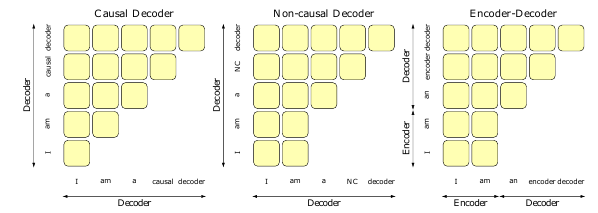
\includegraphics[width=1\columnwidth]{Figure/architectures.png}
\caption{An example of attention patterns in language models, image is taken from~\cite{LLM_Objectives}.}
\label{architectures}
\end{figure}

\subsection{Pre-Training Objectives}
\label{sec:pretrainobjectives}
This section describes LLMs pre-training objectives. For more details see the paper~\cite{LLM_Objectives}. 

\subsubsection{Full Language Modeling}
An autoregressive language modeling objective where the model is asked to predict future tokens given the previous tokens, an example is shown in Figure~\ref{t_objectives}. 

\subsubsection{Prefix Language Modeling}
A non-causal training objective, where a prefix is chosen randomly and only remaining target tokens are used to calculate the loss. An example is shown in Figure~\ref{t_objectives}.

\subsubsection{Masked Language Modeling}
In this training objective, tokens or spans (a sequence of tokens) are masked randomly and the model is asked to predict masked tokens given the past and future context. An example is shown in Figure~\ref{t_objectives}. 

\subsubsection{Unified Language Modeling}
Unified language modeling~\cite{Unified_LM} is a combination of causal, non-causal, and masked language training objectives. Here in masked language modeling, the attention is not bidirectional but unidirectional, attending either left-to-right or right-to-left context.
\begin{figure}[tbp]
\centering
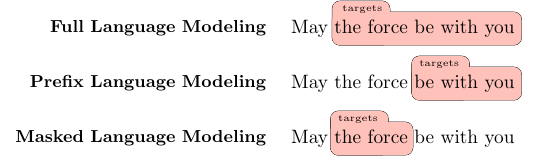
\includegraphics[width=1\columnwidth]{Figure/training_objectives.png}
\caption{An example of language model training objectives, image from~\cite{LLM_Objectives}.}
\label{t_objectives}
\end{figure}

\subsection{Model Adaptation}
This section discusses various model adaptation techniques, where a model is pre-trained on large data and then adapted for downstream tasks. 

\subsubsection{Transfer Learning}
Fine-tuning a pre-trained model with data for the downstream task is known as transfer learning. In this type of model adaptation, the model is initialized with pre-trained weights and updated according to the new data. Some of the LLMs employing this technique are~\cite{T5, mT5, UL2, U-PaLM}. 

\subsubsection{Parameter Efficient Learning}
The parameter efficient learning fine-tunes a few parameters either by adding new parameters to the model or the existing ones. 

\vspace{1mm}
\noindent
\emph{\textbf{Prompt Tuning:}}~\cite{Prompt_Tuning, Prompt_Tuning_2} adds trainable prompt token embeddings as prefixes or free-style to the input token embeddings. During fine-tuning only these embeddings parameters are trained for the downstream task while keeping the rest of the weights frozen.

\vspace{1mm}
\noindent
\emph{\textbf{Prefix Tuning:}}~\cite{Prefix_Tuning} adds task-specific trainable prefix vectors to the transformer layers, where only prefix parameters are fine-tuned, and the rest of the model stays frozen. The input sequence tokens can attend prefixes acting as virtual tokens.    

\vspace{1mm}
\noindent
\emph{\textbf{Adapter Tuning:}} module is an encoder-decoder architecture that is placed either sequential or parallel to the attention and feed-forward layers in the transformer block~\cite{LMAdapter, LMAdapter_2, LMAdapter_3}. Only these layers are fine-tuned, and the rest of the model is kept frozen.  

\subsubsection{Instruction Finetuning}
Instruction tuning is an approach to fine-tuning pre-trained models on instruction formatted data. Instructions generally comprise multiple tasks in plain natural language, guiding the model to respond according to the prompt and the input. The training data consists of an instruction and an input-output pair. More details on formatting instruction data and its various styles are available in~\cite{Survey_LLM}.     

\subsubsection{Alignment Tuning}
LLMs are prone to generate false, biased, and harmful text. Therefore, models are aligned using human feedback to make them helpful, honest, and harmless. Alignment involves asking LLMs to generate unexpected responses and then updating their parameters to avoid such responses~\cite{Survey_LLM}.

\subsubsection{In-context Learning} 
No fine-tuning is involved in this type of model adaptation. The model is shown multiple input-output demonstration pairs to generate a desired input response. This adaptation is similar to a few-shot learning but without requiring any parameter update. More details on formatting demonstrations are available in~\cite{Survey_LLM}. 
 
\subsubsection{Chain-of-thought Prompting}
Chain-of-thought prompting (CoT) is a special case of prompting where demonstrations contain reasoning information aggregated with inputs and outputs so that the model generates outcomes with reasonings. Some examples in literature train LLMs with CoT reasoning, whereas other utilizes LLMs' CoT abilities without fine-tuning. More details on designing prompts are available in~\cite{Survey_LLM}.


\section{Large Language Models}
\label{sec_review}
This section reviews LLMs, briefly describing their architectures, training objectives, pipelines, datasets, and fine-tuning details.      
\subsection{Pre-Trained Models}
\subsubsection{T5~\cite{T5}}
An encoder-decoder model trained on the Colossal Clean Crwal Corpus (C4) dataset with a unified text-to-text training for all NLP problems, shown in Figure~\ref{t5_image}. The model differs from the traditional transformer model~\cite{Transformers}. These changes include no bias in layer normalization, using relative positional embedding, and placing layer normalization outside the residual path. The masked language modeling is used as a pre-training objective where spans (consecutive tokens) were replaced with a single mask instead of separate masks for each token. This type of masking speeds up the training as it produces shorter sequences. After pre-training, the model is fine-tuned using adapter layers~\cite{LMAdapter} for downstream tasks.
\begin{figure}[tbp]
\centering
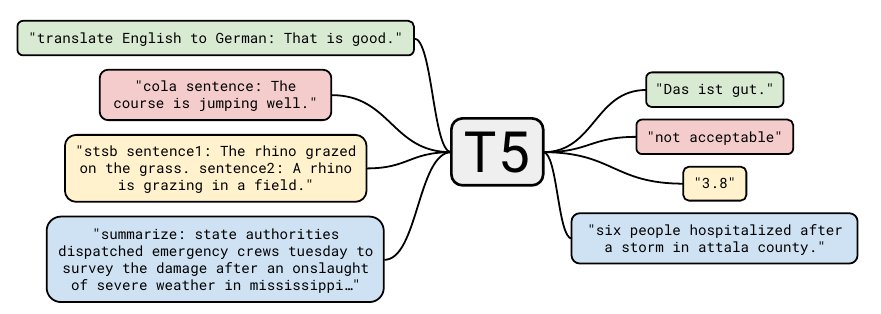
\includegraphics[width=1\columnwidth]{Figure/T5.png}
\caption{Unified text-to-text training example, source image from~\cite{T5}.}
\label{t5_image}
\end{figure}

\subsubsection{mT5~\cite{mT5}}
A multilingual T5 model~\cite{T5} trained on the mC4 dataset with 101 languages. The dataset is extracted from the public common crawl scrape. The model uses GeGLU activation and trains with a vocab size of 250,000 to cover multiple languages. To avoid over-fitting or under-fitting for a language, mT5 employs a data sampling procedure to select samples from all languages. The paper suggests using a small amount of pre-training datasets, including all languages when fine-tuning for a task using English language data. This allows the model to generate non-English outputs.  
%$p(L) \propto \mid L \mid^\alpha$, where $p(L)$ is sampling probability, $L$ is language sampling count, and $\alpha$ controls the sampling probability

\subsubsection{PanGu-$\alpha$~\cite{PanGU_alpha}}
An autoregressive model trained on 1.1TB Chinese data collected from Common Crawl, e-Books, encyclopedia, etc. Additional to the standard transformer model, it has a query layer after stacked transformer layers, example shown in Figure~\ref{pangu_alpha_image}. The purpose of the query layer is to predict the next token. Its structure is similar to the transformer layer but with an additional embedding for the next position in the attention mechanism, given in Eq.~\ref{PanGu_alpha_eq}. The model is trained using MindSpore with five-dimensional parallelism, i.e., data parallelism, op-level model parallelism, pipeline model parallelism, optimizer parallelism, and rematerialization. 
\begin{equation}
a = p_nW_h^qW_h^kTH_L^T
\label{PanGu_alpha_eq}
\end{equation}

\begin{figure}[tbp]
\centering
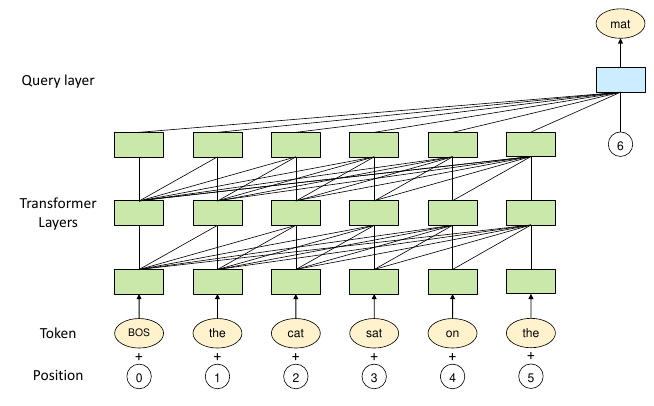
\includegraphics[width=1\columnwidth]{Figure/PanGU_alpha.png}
\caption{The image is the article of~\cite{PanGU_alpha}, showing an example of PanGu-$\alpha$ architecture.}
\label{pangu_alpha_image}
\end{figure}


\subsubsection{CPM-2~\cite{CPM-2}}
Cost-efficient Pre-trained language Models (CPM-2) pre-trains bilingual (English and Chinese) 11B and 198B mixture-of-experts (MoE) models on the WuDaoCorpus~\cite{WuDaoCorpus} dataset. It has an encoder-decoder architecture with a bidirectional encoder and a unidirectional decoder. The tokenization process removes \enquote{\_} white space tokens in the sentencepiece tokenizer. The models are trained with knowledge inheritance, starting with only the Chinese language in the first stage and then adding English and Chinese data. This trained model gets duplicated multiple times to initialize the 198B MoE model. Moreover, to use the model for downstream tasks, CPM-2 experimented with both complete fine-tuning and prompt fine-tuning as in~\cite{LMAdapted} where only prompt-related parameters are updated by inserting prompts at various positions, front, middle, and back. CPM-2 also proposes INFMOE, a memory-efficient framework with a strategy to dynamically offload parameters to the CPU for inference at a 100B scale. It overlaps data movement with inference computation for lower inference time.   

\subsubsection{CodeGen~\cite{CodeGen}}
CodeGen has similar architecture to the PaLM~\cite{PaLM}, i.e., parallel attention, MLP layers, and RoPE embeddings. The model is trained on both natural language and programming language data sequentially (trained on the first dataset, then the second and so on) on the following datasets 1) PILE, 2) BIGQUERY and 3) BIGPYTHON. CodeGen proposed a multi-step approach to synthesizing code. The purpose is to simplify the generation of long sequences where the previous prompt and generated code are given as input with the next prompt to generate the next code sequence. CodeGen opensource a Multi-Turn Programming Benchmark (MTPB) to evaluate multi-step program synthesis.   

\subsubsection{GPT-NeoX-20B~\cite{GPT_NeoX}}
An auto-regressive model that largely follows GPT-3 with a few deviations in architecture design, trained on the Pile dataset without any data deduplication. GPT-NeoX has parallel attention and feed-forward layers in a transformer block, given in Eq.~\ref{GPT-NeoX-20B_eq}, that increases throughput by 15\%. It uses rotary positional embedding~\cite{su2021roformer}, applying it to only 25\% of embedding vector dimension as in~\cite{GPT_J_6B}. This reduces the computation without performance degradation. Opposite to GPT-3, which uses dense and sparse layers, GPT-NeoX-20B uses only dense layers. The hyperparameter tuning at this scale is difficult; therefore, the model chooses hyperparameters from the method~\cite{GPT-3} and interpolates values between 13B and 175B models for the 20B model. The model training is distributed among GPUs using both tensor and pipeline parallelism.   
\begin{equation}
x + Attn(LN_1(x)) + FF(LN_2(x))
\label{GPT-NeoX-20B_eq}
\end{equation}

\subsubsection{UL2~\cite{UL2}}
An encoder-decoder architecture trained using a mixture of denoisers (MoD) objectives. Denoisers include 1) R-Denoiser: a regular span masking, 2) S-Denoiser: which corrupts consecutive tokens of a large sequence and 3) X-Denoiser: which corrupts a large number of tokens randomly. During pre-training, UL2 includes a denoiser token from ${R, S, X}$ to represent a denoising setup. It helps improve fine-tuning performance for downstream tasks that bind the task to one of the upstream training modes. This MoD style of training outperforms the T5 model on many benchmarks.   

\subsubsection{OPT~\cite{OPT}}
It is a clone of GPT-3, developed with the intention to open-source a model that replicates GPT-3 performance. The model was trained using RoBERTa, The Pile, and PushShift.io Reddit datasets. Training of OPT employs dynamic loss scaling ~\cite{S_mixed_precision} and restarts from an earlier checkpoint with a lower learning rate whenever loss divergence is observed. Overall, the performance of OPT-175B models is comparable to the GPT3-175B model.

\subsubsection{GLM-130B~\cite{GLM-130B}}
GLM-130B is a bilingual (English and Chinese) model trained using an auto-regressive mask infilling pre-training objective similar to the GLM~\cite{GLM}. This training style makes the model bidirectional as compared to GPT-3, which is unidirectional. Opposite to the GLM, the training of GLM-130B includes a small amount of multi-task instruction pre-training data (5\% of the total data) along with the self-supervised mask infilling. To stabilize the training, it applies embedding layer gradient shrink. 

\subsubsection{BLOOM~\cite{BLOOM}}
A causal decoder model trained on ROOTS corpus with the aim of open-sourcing an LLM. The architecture of BLOOM is shown in Figure~\ref{bloom_image}, with differences like ALiBi positional embedding, an additional normalization layer after the embedding layer as suggested by the bitsandbytes\footnote{https://github.com/TimDettmers/bitsandbytes} library. These changes stabilize training with improved downstream performance. 

\begin{figure}[tbp]
\centering
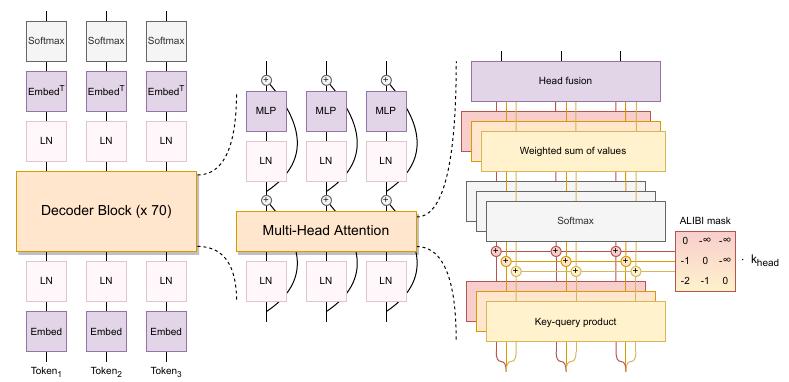
\includegraphics[width=1\columnwidth]{Figure/BLOOM.png}
\caption{The BLOOM architecture example sourced from~\cite{BLOOM}.}
\label{bloom_image}
\end{figure}

\subsubsection{Galactica~\cite{galactica}}
A large curated corpus of human scientific knowledge with 48 million papers, textbooks, lecture notes, millions of compounds and proteins, scientific websites, encyclopedias, and more are trained using metaseq library3, which is built on PyTorch and fairscale~\cite{fairscale}. The model wraps reasoning datasets with $<work>$ token to provide step-by-step reasoning context to the model, which has been shown to improve the performance on reasoning tasks.

\subsubsection{GPT-3}
The architecture of GPT-3 is mostly the same as GPT-2~\cite{GPT-2} but with dense and sparse attention in transformer layers similar to the Sparse Transformer~\cite{sparse_transformer}. The model is trained on data taken from CommonCrawl, Webtext dataset, books corpora, and English-language Wikipedia. Large models can train on larger batch sizes with a lower learning rate; in order to decide the batch size during training, GPT-3 uses the gradient noise scale as in ~\cite{batch_size_selec}. Overall, GPT-3 increases model parameters to 175B showing that the performance of large language models improves with the scale and is competitive with the fine-tuned models.  

\subsubsection{Codex~\cite{codex}}
This LLM is trained on a subset of public Python Github repositories to generate code from docstrings. Computer programming is an iterative process where the programs are often debugged and updated before fulfilling the requirements. Similarly to this, Codex generates 100 versions of a program by repetitive sampling for a given description, which produces a working solution for 77.5\% of the problems passing unit tests.  Its powerful version powers Github Copilot\footnote{https://github.com/features/copilot}.  

\subsubsection{ERNIE 3.0~\cite{ernie3}}
ERNIE 3.0 takes inspiration from multi-task learning to build a modular architecture using Transformer-XL~\cite{dai2019transformer} as the backbone. The universal representation module is shared by all the tasks, which serve as the basic block for task-specific representation modules, which are all trained jointly for natural language understanding, natural language generation, and knowledge extraction. This LLM is primarily focused on the Chinese language, claims to train on the largest Chinese text corpora for LLM training, and achieved state-of-the-art in 54 Chinese NLP tasks.

\subsubsection{Jurassic-1~\cite{lieber2021jurassic}}
A pair of auto-regressive language models, including a 7B-parameter J1-Large model and a 178B-parameter J1-Jumbo model. The Jurassic-1 models are mainly structured on the Transformer decoder module~\cite{Transformers}, while the architecture modifications proposed by GPT-2~\cite{GPT-2} are also incorporated. In particular, the training vocabulary items of Jurassic-1 comprise word pieces, complete words, and multi-word expressions without any word boundaries, where possible out-of-vocabulary instances are interpreted as Unicode bytes. In practice, data collected from publicly available resources are formed in the GPT-3's data structure to train the Jurassic-1 models following the conventional self-supervised auto-regressive training objective. Compared to the GPT-3 counterparts, the Jurassic-1 models apply a more balanced depth-to-width self-attention architecture~\cite{levine2020limits} and an improved tokenizer for a faster prediction based on broader resources, achieving a comparable performance in zero-shot learning tasks and a superior performance in few-shot learning tasks given the ability to feed more examples as a prompt.

\subsubsection{HyperCLOVA~\cite{hyperclova}}
The architecture is the same as that of GPT3~\cite{GPT-3} with morphene aware byte level encoding tokenization step. A large Korean-centric corpus gathered from various sources (see table for details) is trained using Megatron LM. Prompt-based tuning is also applied to enhance performance on downstream tasks. The main objective of training this model is to see how the non-English language model fares compared to universally found English-based LMs.

\subsubsection{Yuan 1.0~\cite{wu2021yuan}}
A large singleton language model with 245B parameters. The Yuan 1.0 is structured as a Transformer~\cite{Transformers}. A Chinese corpus with 5TB of high-quality text is created to train Yuan 1.0 model, where the raw data is collected from Internet resources. A Massive Data Filtering System (MDFS) built on Spark is developed to process the raw data via coarse and fine filtering techniques. To speed up the training of Yuan 1.0 with the aim of saving energy expenses and carbon emissions, a collaborative design of model architecture and large-scale distributed training is introduced. In practice, the Yuan 1.0 model performs well on text classification, Winograd Schema, natural language inference, and reading comprehension tasks.

\subsubsection{Gopher~\cite{gopher}}
It is the largest of six causal decoder LLMs trained on the subsets of MassiveWeb, Books, C4, News, GitHub, and Wikipedia samples from high-quality curated MassiveText. The model is a modified version of Transformer architecture used in~\cite{GPT-2}. The Gopher family of models ranges from 44M to 280B parameters in size to study the effect of \textit{scale} on the LLMs performance. The 280B model beats GPT-3~\cite{GPT-3}, Jurrasic-1~\cite{lieber2021jurassic}, MT-NLG~\cite{mtnlg}, and others on 81\% of the evaluated tasks.

\subsubsection{ERNIE 3.0 TITAN~\cite{ernie3titan}}
ERNIE 3.0 Titan extends ERNIE 3.0 by training a larger model with 26x the number of parameters of the latter. This bigger model outperformed other state-of-the-art models in 68 NLP tasks. LLMs produce text with incorrect facts. In order to have control of the generated text with factual consistency, ERNIE 3.0 Titan adds another task, \textit{Credible and Controllable Generations}, to its multi-task learning setup. It introduces additional self-supervised adversarial and controllable language modeling losses to the pre-training step, which enables ERNIE 3.0 Titan to beat other LLMs in their manually selected Factual QA task set evaluations.

\subsubsection{GLaM~\cite{du2022glam}}
Generalist Language Model (GLaM) represents a family of language models using a sparsely activated mixture-of-experts (MoE) structure~\cite{shazeer2017outrageously,fedus2022switch}. Specifically, the architecture of GLaM is derived from a Decoder-only Transformer~\cite{Transformers}. To gain more model capacity while reducing computation, the experts are sparsely activated where only the best two experts are used to process each input token. The largest GLaM model, GLaM (64B/64E), is about 7$\times$ larger than GPT-3~\cite{GPT-3}, while only a part of the parameters is activated per input token. To effectively compare with GPT-3, the evaluation of GLaM follows the similar zero, one, and few-shot learning protocols as in GPT-3. Specifically, the largest GLaM (64B/64E) model achieves better overall results while consuming only one-third of GPT-3's training energy.

\subsubsection{LaMDA~\cite{thoppilan2022lamda}}
A family of Transformer-based neural language models for dialog ranging from 2B to 137B parameters. The model architecture of LaMDA follows a decoder-only Transformer~\cite{Transformers} language model. LaMDA is pre-trained on public dialog data, public dialog utterances, and public web documents. Particularly, more than 90\% of the pre-training data is in English. Particularly, LaMDA aims to produce responses that exhibit high levels of quality, safety, and groundedness. To achieve this, discriminative and generative fine-tuning techniques are incorporated to enhance the model's safety and quality aspects. As a result, the LaMDA models can be utilized as a general language model performing various tasks.

\subsubsection{MT-NLG~\cite{mtnlg}}
A causal decoder transformer trained on two snapshots of Common Crawl along with some other datasets given in table \ref{datasets}. MT-NLG uses 8-way tensor slicing by Megatron for memory efficiency and 35-way pipeline parallelism using DeepSpeed for compute efficiency to train a 530B model, roughly 3$\times$ GPT-3 model parameters. This model beats GPT-3 on a number of evaluations.

\subsubsection{AlphaCode~\cite{li2022competition}}
A set of large language models designed for competition-level code generation tasks. Basically, the AlphaCode models follow an encoder-decoder transformer architecture~\cite{Transformers} ranging from 300M to 41B parameters. Moreover, the multi-query attention~\cite{shazeer2019fast} is applied to reduce memory and cache costs. Since competitive programming problems highly require deep reasoning and an understanding of complex natural language algorithms, the AlphaCode models are pre-trained on filtered GitHub code in popular languages and then fine-tuned on a new competitive programming dataset named CodeContests. Particularly, the CodeContests dataset mainly contains problems, solutions, and test cases collected from the Codeforces platform\footnote{https://codeforces.com/}. In practice, standard language modeling objectives are used for the pre-training on GitHub code data, while GOLD~\cite{pang2020text} with tempering~\cite{dabre2020softmax} serve as the training objective for the fine-tuning on CodeContests data. To evaluate the performance of AlphaCode, simulated programming competitions are hosted on the Codeforces platform: overall, AlphaCode ranks at the top 54.3\% among over 5000 competitors, where its Codeforces rating is within the top 28\% of recently participated users.

\subsubsection{Chinchilla~\cite{chinchilla}}
A causal decoder trained on the same dataset as the Gopher~\cite{gopher} but with a little different data sampling distribution (sampled from MassiveText). The model architecture is similar to the one used for Gopher, with the exception of AdamW optimizer instead of Adam. Chinchilla identifies the relationship that model size should be doubled for every doubling of training tokens. Over 400 language models ranging from 70 million to over 16 billion parameters on 5 to 500 billion tokens are trained to get the estimates for compute-optimal training under a given budget. The authors train a 70B model with the same compute budget as Gopher (280B) but with 4 times more data. It outperforms Gopher~\cite{gopher}, GPT-3~\cite{GPT-3}, and others on various downstream tasks, after fine-tuning. 


\subsubsection{PaLM}
A causal decoder model trained on a dataset of 780B tokens collected from webpages, books, Wikipedia, news, and others, given in Table~\ref{datasets}. The PaLM has parallel attention and feed-forward layers similar to Eq.~\ref{GPT-NeoX-20B_eq}, speeding up training 15 times faster. Additional changes to the conventional transformer model include SwiGLU activation, RoPE embeddings, multi-query attention that saves computation cost during decoding, and shared input-output embeddings. During training, loss spiking was observed, and to fix it, model training was restarted from a 100 steps earlier checkpoint by skipping 200-500 batches around the spike. Moreover, the model was found to memorize around 2.4\% of the training data at the 540B model scale, whereas this number was lower for smaller models.   

\subsubsection{AlexaTM~\cite{soltan2022alexatm}}
The first multilingual sequence-to-sequence model (20B parameter) is capable of in-context learning. The pre-training data is collected from Wikipedia and mC4 dataset~\cite{mT5} covering 12 programming languages. To enable the AlexaTM 20B model to perform on both spoken and written cases, all data is converted into spoken format via a written-to-spoken formatter. In addition to pre-training on the denoising task, an extra Causal Language Modeling (CLM) task is performed for 20\% of the time to help the model with efficient in-context learning. In practice, the model is asked to continue the input instead of denoising the input once a special CLM token is attached to the beginning of the input.

\subsubsection{Sparrow~\cite{glaese2022improving}}
An information-seeking dialogue agent is trained to gain more helpfulness and correctness with less harm. Two additions are proposed to help human raters judge agent behavior: the first is the specific natural language rules that need raters to rate separately, and the second is to make the agent show proof from sources that support factual claims when collecting opinions about the model's statements. The architecture of the Sparrow models is based on Dialogue Prompted Chinchila 70B~\cite{chinchilla}. Human data is collected for rule violations and per-turn response preferences, which mainly aims to train preference reward models (preference RMs) and a rule reward model (rule RM). In practice, reinforcement learning with advantage actor-critic (A2C)~\cite{mnih2016asynchronous} is used to train the initialized Chinchilla model; the rule RM estimated rule violation rate and the preference RMs estimated per-turn response preferences are jointly optimized. Given experimental data, Sparrow's evidence can support the sampled response for factual questions 78\% of the time. Moreover, Sparrow is highly resistant to human adversarial probing since it only violates the defined rules 8\% of the time when probed.

\subsubsection{U-PaLM~\cite{U-PaLM}}
This method trains PaLM for 0.1\% additional compute with UL2 (also named as UL2Restore) objective~\cite{UL2} using the same dataset and outperforms baseline significantly on various NLP tasks, including zero-shot, few-shot, commonsense reasoning, CoT, etc. Training with UL2R involves converting a causal decoder PaLM to a non-causal decoder PaLM and employing 50\% sequential denoising, 25\% regular denoising, and 25\% extreme denoising loss functions.

\subsubsection{LLaMA~\cite{touvron2023llama}}
A set of foundation language models varying from 7B to 65B parameters. The overall architecture of LLaMA follows the Transformer~\cite{Transformers}, while a few subsequently proposed improvements of normalization~\cite{rmsnorm}, activation~\cite{shazeer2020glu}, and positional embedding~\cite{su2021roformer} operations are incorporated for better performances. About 67\% of LLaMA's pre-training data is collected from English CommonCrawl following the CCNet method~\cite{wenzek2019ccnet}. LLaMA and the associated variants are widely used for parameter-efficient tuning, especially for instruction following tasks.

\subsubsection{PanGu-$\Sigma$~\cite{PanGu_sigma}}
An autoregressive model with parameters copied from PanGu-$\alpha$ and extended to a trillion scale with Random Routed Experts (RRE), the architectural diagram is shown in Figure~\ref{pangu_sigma_image}. RRE is similar to the MoE architecture, with distinctions at the second level, where tokens are randomly routed to experts in a domain instead of using a learnable gating method. The model has bottom layers densely activated and shared across all domains, whereas top layers are sparsely activated according to the domain. This training style allows extracting task-specific models and reduces catastrophic forgetting effects in case of continual learning. 

\begin{figure}[tbp]
\centering
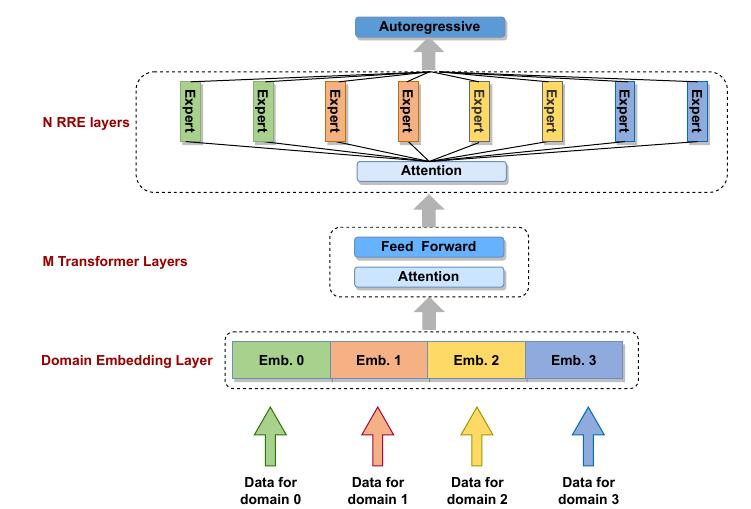
\includegraphics[width=1\columnwidth]{Figure/pangu_sigma.png}
\caption{This example illustrates the PanGu-$\sum$ architecture, as depicted in the image sourced from~\cite{PanGu_sigma}.}
\label{pangu_sigma_image}
\end{figure}


\begin{table*}[!tbhp]

%\renewcommand\tabcolsep{1pt}
\caption{Some of the critical findings and crucial discoveries of each \emph{pre-trained} Large Language Model.}
%\caption{Important findings of pre-trained LLMs}
\begin{tabular}{lc}
\hline \hline
\rowcolor{gray!50} Models & Findings \& Insights\\ \hline \hline
T5 & \begin{tabular}{c} 
\multicolumn{1}{p{15cm}}{\begin{itemize}
\item Encoder and decoder with shared parameters perform equivalently when parameters are not shared
\item Fine-tuning model layers (adapter layers) work better than the conventional way of training on only classification layers
\end{itemize}}
\end{tabular}  \\ \cline{2-2}%\hline

mT5 & \begin{tabular}{c}
\multicolumn{1}{p{15cm}}{\begin{itemize}
\item Large multi-lingual models perform equivalently to single language models on downstream tasks. However, smaller multi-lingual models perform worse
\end{itemize}}
\end{tabular}    \\ \cline{2-2}%\hline

CPM-2 & \begin{tabular}{c}
\multicolumn{1}{p{15cm}}{\begin{itemize}
\item Prompt fine-tuning requires updating very few parameters while achieving performance comparable to full model fine-tuning 
\item Prompt fine-tuning takes more time to converge as compared to full model fine-tuning 
\item Inserting prompt tokens in-between sentences can allow the model to understand relations between sentences and long sequences
\item In an analysis, CPM-2 finds that prompts work as a provider (additional context) and aggregator (aggregate information with the input text) for the model
\end{itemize}}
\end{tabular}  \\ \cline{2-2}%\hline

PanGu-$\alpha$ & \begin{tabular}{c}
\multicolumn{1}{p{15cm}}{\begin{itemize}
\item LLMs are good at a few shot capabilities
\end{itemize}}
\end{tabular} \\ \cline{2-2}%\hline

CodeGen & \begin{tabular}{c}
\multicolumn{1}{p{15cm}}{\begin{itemize}
\item Multi-step prompting for code synthesis leads to a better user intent understanding and code generation
\end{itemize}}
\end{tabular}    \\ \cline{2-2}%\hline

GPT-NeoX-20B & \begin{tabular}{c}
\multicolumn{1}{p{15cm}}{\begin{itemize}
\item Parallel attention + FF layers speed-up training 15\% with the same performance as with cascaded layers
\item Initializing feed-forward output layers before residuals with scheme in~\cite{Mesh_Transformer_JAX} avoids activations from growing with increasing depth and width
\item Training on Pile outperforms GPT-3 on five-shot 
\end{itemize}}
\end{tabular}    \\ \cline{2-2}%\hline

UL2 & \begin{tabular}{c}
\multicolumn{1}{p{15cm}}{\begin{itemize}
\item Mode switching training enables better performance on downstream tasks
\item CoT prompting outperforms standard prompting for UL2  
\end{itemize}}
\end{tabular}    \\ \cline{2-2}%\hline

OPT & \begin{tabular}{c}
\multicolumn{1}{p{15cm}}{\begin{itemize}
\item Restart training from an earlier checkpoint with a lower learning rate if loss diverges
\item Model is prone to generate repetitive text and stuck in a loop
\end{itemize}}
\end{tabular}    \\ \cline{2-2}%\hline

GLM-130B &  \begin{tabular}{c}
\multicolumn{1}{p{15cm}}{\begin{itemize}
\item Pre-training data with a small proportion of multi-task instruction data improves the overall model performance
\end{itemize}}
\end{tabular}    \\ \cline{2-2}%\hline

BLOOM & \begin{tabular}{c}
\multicolumn{1}{p{15cm}}{\begin{itemize}
\item None
\end{itemize}}
\end{tabular}  \\ \cline{2-2}%\hline

Galactica & \begin{tabular}{c}
\multicolumn{1}{p{15cm}}{\begin{itemize}
\item Galactica's performance has continued to improve across validation set, in-domain, and out-of-domain benchmarks, even with multiple repetitions of the corpus, which is superior to existing research on LLMs.
\item A working memory token approach can achieve strong performance over existing methods on mathematical MMLU and MATH benchmarks. It sets a new state-of-the-art on several downstream tasks such as PubMedQA (77.6\%) and MedMCQA dev (52.9\%).
\end{itemize}}
\end{tabular}    \\ \cline{2-2}%\hline

GPT-3 & \begin{tabular}{c}
\multicolumn{1}{p{15cm}}{\begin{itemize}
\item Few-shot performance of LLMs is better than the zero-shot, suggesting that LLMs are meta-learners
\end{itemize}}
\end{tabular}    \\ \cline{2-2}%\hline

Codex & \begin{tabular}{c}
\multicolumn{1}{p{15cm}}{\begin{itemize}
\item This LLM focuses on code evaluations and introduces a novel way of selecting the best code samples.
\item The results indicate it is possible to accurately select code samples using heuristic ranking in lieu of a detailed evaluation of each sample, which may not be feasible or feasible in some situations.
\end{itemize}}
\end{tabular}    \\ \cline{2-2}%\hline

ERNIE 3.0 & \begin{tabular}{c}
\multicolumn{1}{p{15cm}}{\begin{itemize}
\item ERNIE 3.0 shows that a modular LLM architecture with a universal representation module and task-specific representation module helps in finetuning phase.
\item Optimizing the parameters of a task-specific representation network during the fine-tuning phase is an efficient way to take advantage of the powerful pretrained model.
\end{itemize}}
\end{tabular}    \\ \cline{2-2}%\hline

Jurassic-1 & \begin{tabular}{c}
\multicolumn{1}{p{15cm}}{\begin{itemize}
\item The performance of an LLM is highly related to the network size.
\item To improve runtime performance, more operations can be performed
in parallel (width) rather than sequentially (depth).
\item To efficiently represent and fit more text in the same context length, the model uses a larger vocabulary to train a SentencePiece tokenizer without restricting it to word boundaries. This tokenizer improvement can further benefit few-shot learning tasks.
\end{itemize}}
\end{tabular}    %\\ \cline{2-2}%\hline

\\ \hline
\end{tabular}%
\vspace{2mm}
\begin{flushright}
Table Continued on Next Page 
\end{flushright}
 \label{tab:pre_trained_findings}
\end{table*}

%\clearpage
%\pagebreak

\begin{table*}[!tbhp]
%\ContinuedFloat
%\caption{(Continued on next page)}
\begin{tabular}{lc}
\hline \hline
\rowcolor{gray!50}Models & Findings  \& Insights\\ \hline \hline

HyperCLOVA & \begin{tabular}{c}
\multicolumn{1}{p{15cm}}{\begin{itemize}
\item By employing prompt-based tuning, the performances of models can be improved, often surpassing those of state-of-the-art models when the backward gradients of inputs are accessible.
\end{itemize}}
\end{tabular}    \\ \cline{2-2}%\hline

Yuan 1.0 & \begin{tabular}{c}
\multicolumn{1}{p{15cm}}{\begin{itemize}
\item The model architecture that excels in pre-training and fine-tuning cases may exhibit contrasting behavior in zero-shot and few-shot learning.
\end{itemize}}
\end{tabular}    \\ \cline{2-2}%\hline

Gopher & \begin{tabular}{c}
\multicolumn{1}{p{15cm}}{\begin{itemize}
\item Relative encodings enable models to be evaluated for longer sequences than those on which it was trained.
\end{itemize}}
\end{tabular}    \\ \cline{2-2}%\hline

ERNIE 3.0 Titan & \begin{tabular}{c}
\multicolumn{1}{p{15cm}}{\begin{itemize}
\item This LLM builds on top of ERNIE 3.0 and add a self-supervised adversarial loss to distinguish whether a text is generated or the original one. 
\item This distinction ability between real and generate text improves the LLM's performance as compared to ERNIE 3.0.
\end{itemize}}
\end{tabular}    \\ \cline{2-2}%\hline

GLaM & \begin{tabular}{c}
\multicolumn{1}{p{15cm}}{\begin{itemize}
\item The feed-forward component of each Transformer layer can be replaced with a mixture-of-experts (MoE) module consisting of a set of independent feed-forward networks (\emph{i.e.}, the `experts'). By sparsely activating these experts, the model capacity can be maintained while much computation is saved. 
\item By leveraging sparsity, we can make significant strides towards developing high-quality NLP models while simultaneously reducing energy consumption. Consequently, MoE emerges as a robust candidate for future scaling endeavors.
\item The model trained on filtered data shows consistent better performances on both NLG and NLU tasks, where the effect of filtering is more significant on the former tasks.
\item Filtered pretraining corpora plays a crucial role in the generation capability of LLMs, especially for the downstream tasks.
\item The scaling of GLaM MoE models can be achieved by increasing the size or number of experts in the MoE layer. Given a fixed budget of computation, more experts contribute to better predictions.
\end{itemize}}
\end{tabular}    \\ \cline{2-2}% \hline

LaMDA & \begin{tabular}{c}
\multicolumn{1}{p{15cm}}{\begin{itemize}
\item The model can be fine-tuned to learn to call different external information resources and tools.
\end{itemize}}
\end{tabular}    \\ \cline{2-2}%\hline

MT-NLG & \begin{tabular}{c}
\multicolumn{1}{p{15cm}}{\begin{itemize}
\item None.
\end{itemize}}
\end{tabular} \\ \cline{2-2}%\hline

AlphaCode & \begin{tabular}{c}
\multicolumn{1}{p{15cm}}{\begin{itemize}
\item For higher effectiveness and efficiency, a transformer model can be asymmetrically constructed with a shallower encoder and a deeper decoder.
\item To achieve better performances, it is necessary to employ strategies such as massively scaling up sampling, followed by the filtering and clustering of samples into a compact set. 
\item The utilization of novel sampling-efficient transformer architectures designed to facilitate large-scale sampling is crucial.
\item Simplifying problem descriptions can effectively improve the model’s performance.
\end{itemize}}
\end{tabular}    \\ \cline{2-2}%\hline

Chinchilla & \begin{tabular}{c}
\multicolumn{1}{p{15cm}}{\begin{itemize}
\item The experiments that culminated in the development of Chinchilla determined that for optimal computation during training, the model size and the number of training tokens should be scaled proportionately: for each doubling of the model size, the number of training tokens should be doubled as well.
\end{itemize}}
\end{tabular}    \\  \cline{2-2} %\hline
PaLM &  \begin{tabular}{c}
\multicolumn{1}{p{15cm}}{\begin{itemize}
\item English-centric models produce better translations when translating to English as compared to non-English
\item Generalized models can have equivalent performance for language translation to specialized small models
\item Larger models have a higher percentage of training data memorization
\item Performance has not yet saturated even at 540B scale, which means larger models are likely to perform better
\end{itemize}}
\end{tabular}   \\ \cline{2-2}%\hline

AlexaTM & \begin{tabular}{c}
\multicolumn{1}{p{15cm}}{\begin{itemize}
\item Compared to commonly used Decoder-only Transformer models, seq2seq architecture is more suitable for training generative LLMs given stronger bidirectional attention to the context. 
\item An extra Causal Language Modeling (CLM) task can be added to benefit the model with a more efficient in-context learning, especially for few-shot learning tasks. 
\item The key to training powerful seq2seq-based LLMs lies in mixed pre-training, rather than additional multitask training.
\item Placing layernorms at the beginning of each transformer layer can improve the training stability of large models.
\end{itemize}}
\end{tabular}    \\ \cline{2-2}%\hline

Sparrow & \begin{tabular}{c}
\multicolumn{1}{p{15cm}}{\begin{itemize}
\item Reinforcement learning from multi-objective human feedback can be leveraged to train the models, in order to maximize preference rates and minimize rule violations.
\item The judgments of labelers and the alignments with defined rules can help the model generate better responses.
\item Good dialogue goals can be broken down into detailed natural language rules for the agent and the raters.
\item Constructing useful and reliable agents from generative models requires a combination of width and depth: the width aspect enables addressing the complexities of goals and topics; while the depth aspect ensures accurate handling of them.
\item The combination of reinforcement learning (RL) with reranking yields optimal performance in terms of preference win rates and resilience against adversarial probing.
\end{itemize}}
\end{tabular}    \\ \hline %\cline{2-2}



%InstructGPT & \begin{tabular}{c}
%\multicolumn{1}{p{15cm}}{\begin{itemize}
%\item InstructGPT is trained using a novel RLHF technique which produces outputs that are preferred to the outputs from its base model of GPT-3 (175B), despite having 100x fewer parameters.
%\item The human feedback step-trained models show improvements in truthfulness and reductions in toxic output generation while having minimal performance regressions on public NLP datasets
%\end{itemize}}
%\end{tabular}    \\ \hline %\hline

\end{tabular}%

\vspace{2mm}
\begin{flushright}
Table Continued on Next Page 
\end{flushright}
\end{table*}

\begin{table*}[!tbhp]
%\ContinuedFloat
%\caption{}
\begin{tabular}{lc}
\hline \hline
\rowcolor{gray!50}Model & Findings \& Insights \\ \hline \hline

U-PaLM & \begin{tabular}{c}
\multicolumn{1}{p{15cm}}{\begin{itemize}
\item Training with a mixture of denoisers outperforms PaLM when trained further for a few more FLOPs 
\item Training with a mixture of denoisers improves the infilling ability and open-ended text generation diversity
\end{itemize}}
\end{tabular}\\\cline{2-2}% \hline

LLaMA & \begin{tabular}{c}
\multicolumn{1}{p{15cm}}{\begin{itemize}
\item LLaMA is open-source and can be fine-tuned or continually pre-trained to develop new models or instruction-based tools.
\item A few optimizations are proposed to improve the training efficiency of LLaMA, such as efficient implementation of multi-head self-attention and a reduced amount of activations during back-propagation.
\item Training exclusively on public data can also achieve state-of-the-art performance.
\item A constant performance improvement is gained when scaling the model.
\item Smaller models can also realize good performances using more training data and time.  
\end{itemize}}
\end{tabular}    \\ \cline{2-2}%\hline


PanGu-$\Sigma$ & \begin{tabular}{c}
\multicolumn{1}{p{15cm}}{\begin{itemize}
\item Sparse models provide the benefits of large models at a lower computation cost
\item Randomly Routed Experts reduces catastrophic forgetting effects which in turn is essential for continual learning 
\item Randomly Routed Experts allow extracting a domain-specific sub-model in deployment which is cost-efficient while maintaining a performance similar to the original
\end{itemize}}
\end{tabular}    \\ \hline

\end{tabular}%
\end{table*}


\begin{table*}[!tbhp]
\caption{Our several key insights and findings from the study of \emph{instruction-tuned} Large Language Models. }
%\caption{Important findings of instruction-tuned LLMs}

\begin{tabular}{lccl}
\hline \hline
\rowcolor{gray!50}Models & Findings \& Insights \\ \hline \hline

T0 & \begin{tabular}{c}
\multicolumn{1}{p{15cm}}{\begin{itemize}
\item Multi-task prompting enables zero-shot generalization and outperforms baselines    
\item Even a single prompt per dataset task is enough to improve performance
\end{itemize}}
\end{tabular}\\ \cline{2-2}%\hline

WebGPT & \begin{tabular}{c}
\multicolumn{1}{p{15cm}}{\begin{itemize}
\item The answer quality of LLMs can be further improved with human feedback. 
\item To aid the model in effectively filtering and utilizing relevant information, human labelers play a crucial role in answering questions regarding the usefulness of the retrieved documents.
\item Interacting a fine-tuned language model with a text-based web-browsing environment can improve end-to-end retrieval and synthesis via imitation learning and reinforcement learning.
\item Generating answers with references can make labelers easily judge the factual accuracy of answers.%\textbf{}
\end{itemize}}
\end{tabular}    \\ \cline{2-2}%\hline

Tk-INSTRUCT & \begin{tabular}{c}
\multicolumn{1}{p{15cm}}{\begin{itemize}
\item Instruction tuning leads to a stronger generalization of unseen tasks 
\item More tasks improve generalization whereas only increasing task instances does not help 
\item Supervised trained models are better than generalized models 
\item Models pre-trained with instructions and examples perform well for different types of inputs 
\end{itemize}}
\end{tabular}    \\ \cline{2-2}%\hline


mT0 and BLOOMZ & \begin{tabular}{c}
\multicolumn{1}{p{15cm}}{\begin{itemize}
\item Instruction tuning enables zero-shot generalization to the tasks never seen before    
\item Multi-lingual training leads to even better zero-shot generalization for both English and non-English
\item Training on machine-translated prompts improves performance for held-out tasks with non-English prompts  
\item English only fine-tuning on multilingual pre-trained language model is enough to generalize to other pre-trained language tasks
\end{itemize}}
\end{tabular}    \\ \cline{2-2} 

OPT-IML & \begin{tabular}{c}
\multicolumn{1}{p{15cm}}{\begin{itemize}
\item Task size sampling to create a batch with most of the task examples is important for better performance 
\item Only example proportional sampling is not enough, training datasets/benchmarks should also be proportional for better generalization/performance
\item Fully held-out and partially supervised tasks performance improves by scaling tasks or categories whereas fully supervised tasks have no effect

\item Including small amounts i.e. 5\% of pretraining data during fine-tuning is effective 

\item Only 1\% reasoning data improves the performance, adding more deteriorates performance

\item Adding dialogue data makes the performance worse

%\item Meta training for in-context learning degrades performance??? It improves performance for other LLMs though.
\end{itemize}}
\end{tabular}    \\ \cline{2-2}%\hline



Flan & \begin{tabular}{c}
\multicolumn{1}{p{15cm}}{\begin{itemize}
\item Finetuning with CoT improves performance on held-out tasks 
\item Fine-tuning along with CoT data improves reasoning abilities 
\item CoT tuning improves zero-shot reasoning 
\item Performance improves with more tasks 
\item Instruction fine-tuning improves usability which otherwise is challenging for pre-trained models
\item Improving the model's performance with instruction tuning is compute efficient 
\item Multitask prompting enables zero-shot generalization abilities in LM
\end{itemize}}
\end{tabular}\\ \hline %\cline{2-2}
\end{tabular}%
\label{tab:instruction_tuned_findings}
\end{table*}

\begin{table*}[htbp]
\rowcolors{2}{gray!25}{white}
\begin{center}
\caption{Statistics  of  pre-trained LLMs greater than 10B parameters. Pre-training data scale (either in the number of tokens or storage size), and hardware resource costs. In this table, we only include LLMs with a public paper about the technical details. Here, \enquote{Release Time} indicates the date when the corresponding paper was officially released. \enquote{Open Source} means  that the model checkpoints can be publicly accessible. \enquote{Data Cleaning} indicates whether the data cleaning is performed or not. This includes heuristics (Heur), deduplication (Dedup), quality filtering (QF) and privacy filtering (PF).
\enquote{Training Parallelism} indicates distributed training using data parallelism (D), tensor parallelism (T), pipeline parallelism (P), model parallelism (M), optimizer parallelism (OP), and materialization (R). 
}
\label{tab:statistics_pt}
\footnotesize
%\renewcommand\tabcolsep{1pt}
%\hspace*{-5em}
\resizebox{\linewidth}{!}{
\begin{tabular}{llcrccccccccccc}
\toprule
\rowcolor{gray!50}
  &  &   &  & & &   &    & &  &  & &   \\
\rowcolor{gray!50}
\multirow{-2}{*}{\textbf{Models}} & \multirow{-2}{*}{\textbf{\begin{tabular}[c]{@{}c@{}}Release\\ Time\end{tabular}}} & \multirow{-2}{*}{\textbf{\begin{tabular}[c]{@{}c@{}}Open\\ Source\end{tabular}}} & \multicolumn{1}{c}{\multirow{-2}{*}{\textbf{\begin{tabular}[c]{@{}c@{}}Size\\ (B)\end{tabular}}}} & \multirow{-2}{*}{\textbf{\begin{tabular}[c]{@{}c@{}}Base\\ Model\end{tabular}}} & \multirow{-2}{*}{\textbf{\begin{tabular}[c]{@{}c@{}}Steps\\ Trained\end{tabular}}} & \multirow{-2}{*}{\textbf{\begin{tabular}[c]{@{}c@{}}Data/\\ Tokens\end{tabular}}} & \multirow{-2}{*}{\textbf{\begin{tabular}[c]{@{}c@{}}Data\\ Cleaning\end{tabular}}} & \textbf{Hardware} & \multirow{-2}{*}{\textbf{\begin{tabular}[c]{@{}c@{}}Training\\ Time\end{tabular}}} &  \multirow{-2}{*}{\textbf{\begin{tabular}[c]{@{}c@{}}Training\\ Parallelism\end{tabular}}} & \textbf{Library}  \\
\midrule
T5~\cite{T5}   & Oct-2019 &$\checkmark$ & 11   & -   & 1M & 1T & Heur+Dedup & 1024 TPU v3 &  & D+M & Mesh TensorFlow  \\

mT5~\cite{mT5}  & Oct-2020  &$\checkmark$  & 13    & T5  & 1M & 1T & - & -   & -  & - & - \\

{PanGu-$\alpha$}~\cite{PanGU_alpha}   & Apr-2021    &  $\checkmark$  & 200  &  -  &  260k  & 1.1TB  & Heur+Dedup &  2048 Ascend 910  & - & D+OP+P+O+R & MindSpore\\

CPM-2~\cite{CPM-2}    & Jun-2021  & $\checkmark$  & 198   & - & 1M & 2.6TB  & Dedup & - & - & D+M  & JAXFormer   \\

CodeGen~\cite{CodeGen}  & Mar-2022    &  $\checkmark$  & 16   & -  & 650k & 577B  & Heur+Dedup   & TPU v4 & - & D+M & JAXFormer  \\

GPT-NeoX-20B~\cite{black2022gpt} & Apr-2022    & $\checkmark$    & 20   & - & 150k & 825GB & None & 96 40G A100 & - & M & Megatron+DS+PyTorch     \\

UL2~\cite{UL2}  & May-2022    &  $\checkmark$   & 20   & T5  & 2M & 1T & - & 512 TPU v4  & -  & M & JAX+T5X    \\

OPT~\cite{OPT}  & May-2022    & $\checkmark$   & 175   & - &  150k  & 180B  &  Dedup   & 992 80G A100  & -  & D+T & Megatron   \\

GLM~\cite{GLM-130B}  & Oct-2022 & $\checkmark$   & 130   & - & - & 400B   & -  & 768 40G A100    & 60d  & M & -    \\

BLOOM~\cite{BLOOM}    & Nov-2022  & $\checkmark$  & 176   & -   & - & 366B & Dedup+PR  & 384 80G A100    & 105d  &  D+T+P  & Megatron+DS    \\

Galactica~\cite{galactica} & Nov-2022    & $\checkmark$ & 120   & - & 225k & 106B & Dedup  &  128 80GB A100   & -  & - & Metaseq    \\

GPT-3~\cite{GPT-3}    & May-2020   & $\times$ & 175   & - & - & 300B & -  & -   & -  & - & -       \\

Codex~\cite{codex}    & Jul-2021 & $\times$   & 12    & GPT-3 & - & 100B & Heur & -   & -  & -    & - \\

ERNIE 3.0~\cite{ernie3}    & Jul-2021  & $\times$  & 10  & - & 120k$^*$ & 375B & Heur+Dedup & 384 V100   & -  & M$^*$ & PaddlePaddle    \\

Jurassic-1~\cite{lieber2021jurassic}   & Aug-2021 & $\times$  & 178      & - & - & 300B   & -  & 800 GPU & -  & D+M+P    & Megatron+DS       \\

HyperCLOVA~\cite{hyperclova}   & Sep-2021 & $\times$   & 82 & -  & - &  300B  & Clf+Dedup+PF & 1024 A100   & 13.4d  & M  & Megatron      \\

Yuan 1.0~\cite{wu2021yuan}   & Oct-2021  & $\times$  & 245   & -  & 26k$^*$ &  180B  &  Heur+Clf+Dedup  & 2128 GPU  &  -  & D+T+P & - \\

% WebGPT~\cite{nakano2021webgpt}   & Dec-2021  &$\times$  & 175   & GPT-3   & - & -  & - & -  & -   & -  & -   \\

Gopher~\cite{gopher}   & Dec-2021 & $\times$   & 280 & ERNIE-3.0 & - & 300B   & QF+Dedup  & 4096 TPU v3 & 920h  & D+M    & JAX+Haiku        \\

ERNIE 3.0 Titan~\cite{ernie3titan}   & Dec-2021 & $\times$   & 260  & -  & - &  300B  & Heur+Dedup &  V100+Ascend 910  & -  & D+M+P+D* & PaddlePaddle  \\

GLaM~\cite{du2022glam} &Dec-2021  &$\times$    & 1200  & -   & 600k$^*$  & 600B   & Clf  & 1024 TPU v4 & -  & M & GSPMD       \\

LaMDA~\cite{thoppilan2022lamda}    & Jan-2022   & $\times$ & 137      & - & 3M & 2.81T  & Filtered  & 1024 TPU v3 & 57.7d & D+M    & Lingvo    \\

MT-NLG~\cite{mtnlg}   & Jan-2022    & $\times$   & 530   & - & - & 270B & - & 4480 80G A100   & -  & D+T+P    & Megatron+DS       \\

AlphaCode~\cite{li2022competition}    & Feb-2022  &$\times$  & 41    & -   & 205k & 967B & Heur+Dedup & TPU v4  & -  &M   & JAX+Haiku       \\

Chinchilla~\cite{chinchilla}   & Mar-2022    & $\times$    & 70   & - & - & 1.4T  & QF+Dedup  & TPUv3/TPUv4   & -  & -    & JAX+Haiku        \\

PaLM~\cite{PaLM} & Apr-2022    & $\times$ & 540 & - &  255k  & 780B  & Heur & 6144 TPU v4  & - & D+M & JAX+T5X\\

AlexaTM~\cite{soltan2022alexatm}  & Aug-2022 &$\times$   & 20  & -  & 500k  & 1.1T   & Filtered  & 128 A100    & 120d  & M & DS      \\

Sparrow~\cite{glaese2022improving}  & Sep-2022 &$\times$    & 70    & Chinchilla   & - & -  & -  & 64 TPU v3   & -  & M    & -       \\

U-PaLM~\cite{U-PaLM}   & Oct-2022    & $\times$ & 540   & PaLM & 20k & - & -   & 512 TPU v4  & 5d    & - & - \\

LLaMA~\cite{touvron2023llama}    & Feb-2023 & $\checkmark$   & 65      & - & 350k & 1.4T & Heur+Dedup   & 2048 80G A100 & 21d   & D+M & xFormers     \\

{PanGu-$\Sigma$}~\cite{PanGu_sigma}    & Mar-2023  & $\times$  & 1085 & {PanGu-$\alpha$} & -  & 329B & -  & 512 Ascend 910   & 100d  & D+OP+P+O+R & MindSpore  \\
%\multirow{-25}{*}{\begin{tabular}[c]{@{}c@{}}Closed\\ Source\end{tabular}} & \multirow{-18}{*}{\begin{tabular}[c]{@{}c@{}}Publicly\\ Available\end{tabular}} &
\bottomrule
\end{tabular}
} 
\end{center}
\end{table*}





\begin{table*}[tbp]
\rowcolors{2}{gray!25}{white}
\centering
\caption{Statistics of instruction tuned LLMs greater than 10B parameters. All abbreviations are the same as Table~\ref{tab:statistics_pt}}
\footnotesize
\resizebox{\linewidth}{!}{
\begin{tabular}{llcrccccccccccc}
\toprule
\rowcolor{gray!50}
  &  &   &  & & &   &    & &  &  & &   \\
\rowcolor{gray!50}
\multirow{-2}{*}{\textbf{Models}} & \multirow{-2}{*}{\textbf{\begin{tabular}[c]{@{}c@{}}Release\\ Time\end{tabular}}} & \multirow{-2}{*}{\textbf{\begin{tabular}[c]{@{}c@{}}Open\\ Source\end{tabular}}} & \multicolumn{1}{c}{\multirow{-2}{*}{\textbf{\begin{tabular}[c]{@{}c@{}}Size\\ (B)\end{tabular}}}} & \multirow{-2}{*}{\textbf{\begin{tabular}[c]{@{}c@{}}Base\\ Model\end{tabular}}}  & \multirow{-2}{*}{\textbf{\begin{tabular}[c]{@{}c@{}}Steps\\ Trained\end{tabular}}} & \multirow{-2}{*}{\textbf{\begin{tabular}[c]{@{}c@{}}Data/\\ Tokens\end{tabular}}} & \multirow{-2}{*}{\textbf{\begin{tabular}[c]{@{}c@{}}Data\\ Cleaning\end{tabular}}} & \textbf{Hardware} & \multirow{-2}{*}{\textbf{\begin{tabular}[c]{@{}c@{}}Training\\ Time\end{tabular}}} &  \multirow{-2}{*}{\textbf{\begin{tabular}[c]{@{}c@{}}Training\\ Parallelism\end{tabular}}} & \textbf{Library}  \\
\midrule

T0~\cite{T0}   & Oct-2021  & $\checkmark$ & 11    & T5  & -  & 250B &  - & 512 TPU v3  & 270h   & - & - \\

WebGPT~\cite{nakano2021webgpt}   & Dec-2021  &$\times$  & 175   & GPT-3   & -  & - & -  & -   & -  &  - &  -  \\

Tk-Instruct~\cite{Tk-INSTRUCT}  & Apr-2022   & $\checkmark$ & 11    & T5  & 1000  & - & - & 256 TPU v3   & 4h  & -  & Google T5   \\

mT0~\cite{mT0}  & Nov-2022  & $\checkmark$  & 13    & mT5 & -  & - & - & -  & -   & -  & - \\

OPT-IML~\cite{OPT_IML}  & Dec-2022  & $\checkmark$ & 175   & OPT & 8k  & 2B & Dedup & 128 40G A100   & - & D+T & Megatron    \\

Flan-U-PaLM~\cite{Flan}  & Oct-2022  & $\times$ & 540   & U-PaLM  & 30k  & - & -  & 512 TPU v4 & - & - & JAX+T5X  \\


%\multirow{-25}{*}{\begin{tabular}[c]{@{}c@{}}Closed\\ Source\end{tabular}} & \multirow{-18}{*}{\begin{tabular}[c]{@{}c@{}}Publicly\\ Available\end{tabular}} &
\bottomrule
\end{tabular}}
\label{tab:statistics_it}
\end{table*}




\subsection{Instruction-Tuned Models}

\subsubsection{T0}
Similar to Flan~\cite{Flan}, T0 fine-tunes the LM-adapted T5 model~\cite{LMAdapted} with multi-task instruction prompts. To train the model, T0 designs various prompt templates to convert different datasets into prompts. The model trained with explicit multi-task prompting improves zero-shot performance, outperforming models 6 to 16 times larger in size.  

\subsubsection{WebGPT~\cite{nakano2021webgpt}}
A set of fine-tuned GPT-3~\cite{GPT-3} models that can answer long-form questions in a text-based web-browsing environment. During browsing, the models must collect references to support their answers in order to exploit easier human evaluation. In addition to the Q\&A data in the ELI5 dataset~\cite{fan2019eli5}, two more types of data, \emph{demonstrations} of humans and \emph{comparisons} between two model-generated answers, are collected for training. Using human labelers' feedback on whether the retrieved information is useful to answer the given inputs, the data is tested with four usages: behavior cloning, reward modeling, reinforcement learning, and rejection sampling. Practically, the combination of behavior cloning and rejection sampling contributes to the best-performing model containing 175B parameters. To evaluate the performance of the WebGPT model, the model's answers are compared with the human demonstrators' written ones, the highest-voted answers in ELI5~\cite{fan2019eli5}, and the adversarial short-form questions and answers in the TruthfulQA~\cite{lin2021truthfulqa} dataset.

\subsubsection{Tk-INSTRUCT~\cite{Tk-INSTRUCT}}
Tk-INSTRUCT instruction fine-tunes T5 model on self-proposed SUPER-NATURALINSTRUCTIONS dataset of 1616 different NLP tasks. To analyze the generalization capabilities of Tk-INSTRUCT, the model is evaluated on unseen tasks with a few examples as ground-truth in-context instructions. The model outperforms GPT-3 and Instruct-GPT by large margins, although it is smaller in size 11B, opposite to 175B.   

\subsubsection{mT0 and BLOOMZ~\cite{mT0andBLOOMZ}}
This method fine-tunes BLOOM and T0 using a multilingual multi-task prompt dataset. It creates a new dataset named xP3, adding 46 different language datasets with new tasks not present previously in P3. Training with this dataset improves zero-shot generalization for both English and non-English. This also leads to better generalization on held-out tasks.    

\begin{figure}[!tbp]
\centering
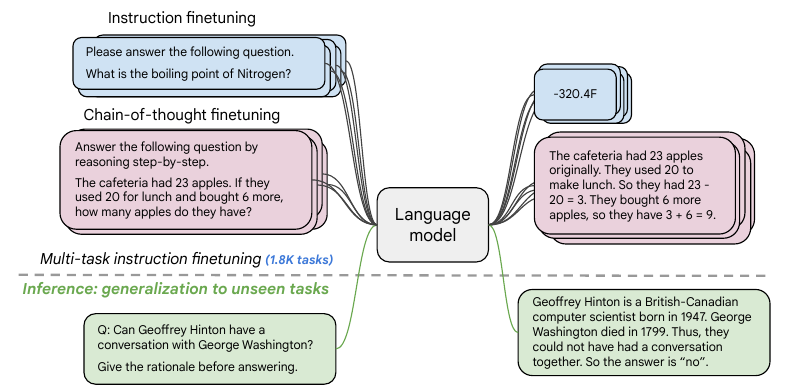
\includegraphics[width=1\columnwidth]{Figure/Flan.png}
\caption{An example image shows an instance of the Flan training paradigm, taken from~\cite{Flan}.}
\label{flan_image}
\end{figure}
\subsubsection{OPT-IML~\cite{OPT_IML}}
An instruction-tuned OPT model, trained on instruction meta-learning benchmark of 2000 NLP tasks that is a combination of 8 meta-datasets including, Super-NaturalInstructions, PromptSource, FLAN, and others as given in Table~\ref{datasets}. For computational efficiency, OPT-IML utilizes the maximum sequence length of 2048 tokens by packing multiple instances together, separated by the $<eos>$ token during training. It employs a masking mechanism to separate instances in a sequence to avoid attending tokens from different instances. Overall, OPT-IML outperforms baseline model OPT with instruction-finetuning on zero and few-shot generalization abilities.

\subsubsection{Flan~\cite{Flan}}
Fine-tuning language models (Flan), fine-tunes T5, PaLM, and UPaLM with 1836 instruction tasks taken from Muffin (80 tasks), T0-SF (193 tasks), NIV2 (1554 tasks), and CoT (taken from nine datasets), as shown in Figure~\ref{flan_image}. Instruction fine-tuning improves the model performance significantly with minimal computing, only 0.2\% of the total pre-training compute in the case of PaLM 540B. Flan also suggests that adding more instruction fine-tuning tasks with CoT reasoning data will likely improve the performance further.   








% % We will externalize the figures
% \usepgfplotslibrary{external}
% \tikzexternalize

% \pgfplotsset{width=18cm,compat=1.9}
% \begin{figure*}[!tbp]
% \centering
% \pgfplotstableread{
% Group  Posttest LLMs Val color
% 2019 1 {T5} 1 .1
% 2020  2  {GPT-3, GShard, mT5} 3 .1
% 2021  1 {PanGu-$\alpha$, PLUG, Codex, ERNIE 3.0, Jurassic-1, CPM-2, FLAN, Yuan 1.0, T0, HyperCLOVA, Anthropic, WebGPT, ERNIE 3.0 TITAN, Gopher, GLaM} 7 .1
% 2022  2  {InstructGPT, CodeGen, MT-NLG, LaMBDA, AlphaCode, Chinchilla, UL2, PaLM, YaLM, OPT, GPT-NeoX-20B, Tk-Instruct, Cohere, GLM, AlexaTM, WeLM, Sparrow, Flan-T5, Flan-PaLM, Luminous, NLLB, BLOOM, mT0, BLOOMZ, Galacitca, OPT-IML, ChatGPT} 10.5 .1
% 2023 1 {CodeGeeX, Pythia, Vicuna, PanGu-$\sum$, Bard, LLaMA, GPT-4} 4 .1
% }\datatable

% \begin{tikzpicture}
% \begin{axis}[
%     xtick=data,
%     enlargelimits=.1,
%     symbolic x coords = {2019,2020,2021,2022,2023},
%     ytick distance=1,
%     ymajorticks=false,
%     scale only axis,
%     xticklabel style={anchor=north,align=center},
%     xticklabels={2019,2020,2021,2022,2023},
%     enlarge y limits=0.75, % Adjust this value as needed
% ]
% \addplot[%
%     scatter=true,
%     only marks,
%     point meta=\thisrow{color},
%     fill opacity=0.1,
%     text opacity=1,
%     visualization depends on={10*\thisrow{Val} \as \perpointmarksize},
%     visualization depends on={\thisrow{Val} \as \Val},
%     scatter/@pre marker code/.append style={
%         /tikz/mark size=\perpointmarksize
%     },
%     nodes near coords*={
%         \pgfplotstablegetelem{\coordindex}{LLMs}\of{\datatable}%
%         \pgfplotsretval%
%     },
%     nodes near coords style={
%         text=black,
%         font=\sffamily,
%         anchor=center,
%         align=center,
%         text width=3cm
%     },
% ]
% table [x={Group},y={Posttest}] {\datatable};      
% \end{axis}
% \end{tikzpicture}
% \caption{Bubble Chart}
% \label{fig:bubblellms}
% \end{figure*}

% \pgfplotsset{width=9cm,compat=1.9} 
% \begin{figure}
%     \centering
%     \begin{tikzpicture}
%     \begin{axis}[
%     	x tick label style={
%     		/pgf/number format/1000 sep=},
%     	ylabel=Year,
%     	enlargelimits=0.05,
%         ymin=1,
%     	legend style={at={(0.5,-0.1)},
%     	anchor=north,legend columns=-1},
%         ybar interval=0.4,
%         ymajorgrids=false,
%         xticklabels={2023,2022,2021,2020,upto 2019,2018},
%     ]
    
%     \addplot[fill=green!30,draw=green] 
%     	coordinates {(2023,4) (2022,14) (2021,4) (2020,1) (2019,1) (2018,2)};
    
%      \addplot[fill=blue!30,draw=blue] 
%     	coordinates {(2023,3) (2022,13) (2021,11) (2020,2) (2019,0) (2018,2)};
%     \legend{Open,Closed}
%     \end{axis}
%     \end{tikzpicture}
%     \caption{Caption}
%     \label{fig:barllms}
% \end{figure}
\section{Findings}
\label{sec:Findings}
Training a billion-scale model is difficult as compared to a smaller model. LLMs are prone to various instabilities during training, such as hardware failure and instability. Other than this, LLMs exhibit different behaviors such as emergent abilities, improved zero-shot, few-shot, and reasoning abilities. Researchers report these essential details in their papers for results reproduction and field progress. We identify critical information in Table~\ref{tab:pre_trained_findings}~and~\ref{tab:instruction_tuned_findings} such as architecture, training strategies, and pipelines that improve LLMs' performance or other abilities acquired because of changes mentioned in section~\ref{sec_review}.  
\section{Model Configurations}
\label{Model_Configurations_}

We provide different statistics of pre-trained and instruction-tuned models in this section. This includes information such as release time, base model, steps trained, parallelism, etc in Table~\ref{tab:statistics_pt} and Table~\ref{tab:statistics_it}. Architecture details of pre-train LLMs are available in Table~\ref{tab:arch_details}. Providing these details for instruction-tuned models is not necessary because it fine-tunes pre-trained models for instruction datasets. Hence, architectural details are the same as the baselines. Moreover, detailed optimization settings for various LLMs are available in Table~\ref{tab:opt_details}.   


\begin{table*}[tbp]
\rowcolors{2}{gray!25}{white}

    \centering
    \caption{Various architecture details of LLMs. Here, \enquote{PE} denotes position embedding, \enquote{\#L} denotes the number of layers, \enquote{\#H} denotes the number of attention heads, $d_{model}$ denotes the size of hidden states}
    \label{tab:arch_details}
\resizebox{\linewidth}{!}{
    \begin{tabular}{lcrcccccrrrr}
    \toprule
 \rowcolor{gray!50}
        \textbf{Models}&\textbf{Category}&\begin{tabular}[c]{@{}c@{}}\textbf{Training}\\ \textbf{Objective}\end{tabular}&\textbf{Vocab }&\textbf{Tokenizer}&\textbf{Norm}&\textbf{PE}&\textbf{Activation}&\textbf{Bias}& \textbf{\#L}& \textbf{\#H}&\textbf{$d_{model}$} \\
\midrule

T5~(11B)&Enc-Dec&Span Corruption&32k&SentencePiece&Pre-RMS &Relative&ReLU&$\times$&24&128&1024\\
mT5~(13B)&Enc-Dec&Span Corruption&250k&SentencePiece&Pre-RMS &Relative&ReLU& - & - & - &-\\
PanGu-$\alpha$~(200B)&Causal-Dec&Next Token&40k&BPE&Layer&-&-&-&64&128&16384\\
CPM-2~(198B)&Enc-Dec&Span Corruption&250k&SentencePiece&Pre-RMS &Relative&ReLU& - & 24 & 64 &-\\

CodeGen~(16B)&Causal-Dec&Next Token&-&BPE&Layer&RoPE&-&-&34&24&-\\

GPT-NeoX-20B & Causal-Dec & Next Token & 50k & BPE & Layer & Rotary & GeLU & $\checkmark$ & 44 & 64 & - \\

UL2~(20B) & Enc-Dec & MoD & 32k & SentencePiece & - & - & - & - & 64 & 16 & 4096\\

OPT~(175B)&Causal-Dec&Next Token&-&BPE&-&-&ReLU&$\checkmark$&96&96&-\\

GLM (130B) & Non-Causal-Dec & AR Blank Infilling & 130k & SentencePiece & Deep & RoPE & GeGLU & \checkmark & 70 & 96 & 12288\\

BLOOM~(176B)&Causal-Dec&Next Token&250k&BPE&Layer&ALiBi&GeLU&$\checkmark$&70&112&14336\\

Galactica~(120B)&Causal-Dec&Next Token&50k&BPE+custom&Layer&Learned&GeLU&$\times$&96&80&10240\\

GPT3~(175B) & Causal-Dec & Next Token & - & - & Layer & Learned & GeLU & \checkmark & 96 & 96 & 12288\\

Jurassic-1~(178B)&Causal-Dec&Next Token &256k &SentencePiece$^*$ &Pre-Layer&Learned&GeLU &$\checkmark$ &76 &96&13824 \\

LLaMA~(65B)&Causal-Dec&Next Token& - &BPE &Pre-RMS&RoPE&SwiGLU&-&80&64&8192\\

HyperCLOVA~(82B)&Causal-Dec&Next Token& - &BPE* &Pre-Layer&Learned&GeLU&-&64&80&10240\\

Codex~(12B)&Causal-Dec&Next Token& - &BPE+ &Pre-Layer&Learned&GeLU&-&96&96&12288\\

ERNIE 3.0~(10B)&Causal-Dec&Next Token& - &WordPiece &Post-Layer&Relative&GeLU&-&48&64&4096\\

ERNIE 3.0 Titan~(260B)&Causal-Dec&Next Token& - &WordPiece &Post-Layer&Relative&GeLU&-&48&192&12288\\

PaLM~(540B)&Causal-Dec&Next Token&256k&SentencePiece&Layer&RoPE&SwiGLU&$\times$&118&48&18432\\

U-PaLM~(540B)&Non-Causal-Dec&MoD&256k&SentencePiece&Layer&RoPE&SwiGLU&$\times$&118&48&18432\\


PanGu-$\Sigma$~(1085B) & Causal-Dec & Next Token & - & BPE & Fused Layer & - & FastGeLU & - & 40 & 40 & 5120 \\
CPM-2~(198B)&Enc-Dec&Span Corruption&250k&SentencePiece&Pre-RMS &Relative&ReLU& - & 24 & 64 &-\\

MT-NLG~(530B)&Causal-Dec&Next Token&50k&BPE&Pre-Layer&Learned&GeLU&$\checkmark$&105&128&20480\\
Gopher~(280B)&Causal-Dec&Next Token&32k&SentencePiece&Pre-RMS&Relative&GeLU&$\checkmark$& 80&128&16384 \\
Chinchilla~(70B)&Causal-Dec&Next Token&32k&SentencePiece-NFKC&Pre-RMS&Relative&GeLU&$\checkmark$& 80&64&8192\\
LaMDA~(137B)&Causal-Dec&Next Token &32k &BPE &Layer &Relative &GeGLU&-&64&128&8192\\
Yuan 1.0~(245B)&Causal-Dec&Next Token& - &- &-&-&-&-&76&-&16384\\
WebGPT~(175B)&Causal-Dec&BC+RM &- &BPE &Pre-Layer & Learned & GeLU & \checkmark & 96 & 96 & 12288\\
GLaM~(1.2T)&MoE-Dec&Next Token& 256k &SentencePiece &Layer&Relative&GeLU&$\checkmark$&64&128&32768\\
InstructGPT~(6B)&Causal-Dec&RM+PPO& - &BPE &Pre-Layer&Learned&GeLU&-&32&32&4096\\
AlphaCode~(41B)&Enc-Dec&Next Token%+ Masked language modeling loss
& 8k &SentencePiece &-&-&-&-&64&128&6144\\
AlexaTM~(20B)&Enc-Dec&Denoising& 150k &SentencePiece &Pre-Layer&Learned&GeLU&$\checkmark$&78&32&4096\\
Sparrow~(70B)&Causal-Dec&Pref.\&Rule RM&32k&SentencePiece-NFKC&Pre-RMS&Relative&GeLU&$\checkmark$&16$^*$&64&8192\\
\bottomrule
\end{tabular}}
\end{table*}

\begin{table*}[tbp]
\rowcolors{2}{gray!25}{white}
\centering
\caption{Detailed optimization settings of pre-trained LLMs}
\label{tab:opt_details}
\resizebox{\linewidth}{!}{
\begin{tabular}{lrrcccccccc}
\toprule
\rowcolor{gray!50}
\textbf{Models}          & \textbf{Batch Size} & \begin{tabular}[r]{@{}r@{}}\textbf{Sequence}\\\textbf{Length}\end{tabular}& \begin{tabular}[r]{@{}r@{}}\textbf{Learning}\\ \textbf{Rate}\end{tabular}   & \textbf{Warmup} & \textbf{Decay Method}   & \textbf{Optimizer}                              & \begin{tabular}[l]{@{}l@{}}\textbf{Precision}\\ \textbf{Type}\end{tabular} & \begin{tabular}[l]{@{}l@{}}\textbf{Weight}\\ \textbf{Decay}\end{tabular}                & \begin{tabular}[l]{@{}l@{}}\textbf{Grad}\\ \textbf{Clip}\end{tabular} & \textbf{Dropout} \\ \midrule
T5~(11B) & 2$^{11}$ & 512 & 0.01 & no  & inverse square root     & AdaFactor & - & - & - & 0.1              \\
mT5~(13B) & 1024& 1024 & 0.01 & -  & inverse square root     & AdaFactor & - & - & - & 0.1              \\
PanGu-$\alpha$~(200B)   & - & 1024 & 2e-5 & - & -  & - & 0.1  & - & -                \\
CPM-2~(198B) & 1024& 1024 & 0.001 & -  & -    & AdaFactor & - & - & - & 0.1              \\
CodeGen~(16B) & 2M& 2048 & 5e-5 & yes  & cosine    & Adam & - & 0.1 & 1.0 & -              \\
GPT-NeoX-20B & 1538  & 2048 & 0.97e-5 & yes & cosine & AdamW & FP16  & 0.01 & 1.0 & 0.0              \\
UL2~(20B) & 1024  & 1024 & - & - & inverse square root & - & -  & - & - & 0.0              \\
OPT~(175B) & 2M  & 2048 & 1.2e-4 & - & linear & AdamW & FP16 & 0.1  & 1.0 & 0.1              \\

GLM~(130B) & 4224  & 2048 & 8e-5  & yes & cosine    & AdamW & FP16 & 0.1 & 1.0 & 0.1              \\

BLOOM~(176B) & 2048  & 2048 & 6e-5 & yes  & cosine    & Adam  & BF16 & 0.1 & 1.0 & 0.0              \\

Galactica~(120B) & 2M & 2048 & 7e-6 & yes & linear decay to 10\%    & AdamW  & - & 0.1  & 1.0 & 0.1              \\

GPT3~(175B) & 32K  & - & 6e-5 & yes & cosine    & Adam & FP16 & 0.1 & 1.0  & -                \\

Codex~(12B) & -  & - & 6e-5 & yes & cosine    & Adam & FP16 & 0.1 & -  & -                \\

ERNIE 3.0~(12B) & 6144  & 512 & 1e-4 & yes & linear    & Adam & - & 0.01 & -  & -                \\

Jurassic-1~(178B) & 3.2M &2048 & 6e-5 & yes & cosine & Adam & FP16 & 0.1 & 1.0 & -                \\

HyperCLOVA~(82B) & 1024  & - & 6e-5 & - & cosine    & AdamW & - & yes & -  & -                \\

Yuan 1.0~(245B) & $<$10M &2048 & 1.6e-4 & yes & cosine decay to 10\%    & Adam & -  & 0.1 & - & -                \\

Gopher~(280B) & 3M  & 2048 & 4e-5 & yes & cosine decay to 10\%    & Adam  & BF16  & -   & 0.25  & -                \\

ERNIE 3.0 Titan~(260B)  & -  & 512 & 1e-4 & yes & linear    & Adam & FP16 & 0.1 & 1.0  & -      \\

GLaM~(1.2T) & 1M &1024 & 0.01 & - & inverse square root   & Adafactor & FP32+BF16  & - & 1.0 & 0.0                \\

LaMDA~(137B) & 256K  & - & - & - & -  & - & - & - & - &-               \\

MT-NLG~(530B) & 1920  & 2048 & 5e-5 & yes & cosine decay to 10\%   & Adam & BF & 0.1 & 1.0  & - \\

AlphaCode~(41B) & 2048 &1536+768 & 1e-4 &yes& cosine decay to 10\%   & AdamW & BF16  &0.1 & 1.0 &-               \\

Chinchilla~(70B) & 1.5M & 2048 & 1e-4 & yes & cosine decay to 10\% & AdamW & BF16 & - & - & -                \\

PaLM~(540B) & 2048 & 2048 & 0.01 & - & inverse square root & Adafactor  & -  & $lr^2$ & 1.0 & 0.0              \\

AlexaTM~(20B) & 2M &1024 & 1e-4 &- & linear decay to 5\%   & Adam & BF16  &0.1 & - &0.15              \\

Sparrow~(70B)& RM: 8+16, RL:16 &- & 2e-6 &yes & cosine decay to 10\%   & Adam+Adafactor & BF16  &- & 1.0 &0.0 \\

U-PaLM~(540B) & 32 & 2048 & 1e-4 & - & cosine & Adafactor  & -  & - & - & -              \\

LLaMA~(65B) & 4M &- & 1.5e-4 & yes & cosine decay to 10\%    & AdamW & -  & 0.1 & 1.0 & -                \\

PanGu-$\Sigma$~(1.085T) & 512  & 1024 & 2e-5 & yes & - & Adam & mixed & - & - & -                \\
\bottomrule
\end{tabular}
}
\end{table*}


\begin{table*}[tbp]
\rowcolors{2}{gray!25}{white}

\centering
\caption{We provide the detailed optimization settings of instruction-tuned LLMs}
\resizebox{\linewidth}{!}{
\begin{tabular}{lrrcccccccc}
\toprule
\rowcolor{gray!50}\textbf{Models}          & \textbf{Batch Size} & \begin{tabular}[r]{@{}r@{}}\textbf{Sequence}\\\textbf{Length}\end{tabular}& \begin{tabular}[r]{@{}r@{}}\textbf{Learning}\\ \textbf{Rate}\end{tabular}   & \textbf{Warmup} & \textbf{Decay Method}   & \textbf{Optimizer}                              & \begin{tabular}[l]{@{}l@{}}\textbf{Precision}\\ \textbf{Type}\end{tabular} & \begin{tabular}[l]{@{}l@{}}\textbf{Weight}\\ \textbf{Decay}\end{tabular}                & \begin{tabular}[l]{@{}l@{}}\textbf{Grad}\\ \textbf{Clip}\end{tabular} & \textbf{Dropout} \\ \midrule
T0~(11B) & 1024 & 1280 & 1e-3 & -  & -   & AdaFactor & - & - & - & 0.1             \\
WebGPT~(175B) & BC:512, RM:32  & - & 6e-5 & - & -    & Adam & - & - & -  & -                \\
Tk-Instruct~(11B) & 1024 & - & 1e-5  & -  & constant  & - & BF16 & - & - & -             \\
mT0~(11B) & - & - & - & -  & - & - & - & - & - & -             \\
OPT-IML~(175B) & 128 & 2048 & 5e-5 & yes  & linear   & Adam & - & - & 1.0 & 0.1             \\
%InstructGPT~(6B) & SFT:32  & 2000 & 9.65e-6 & no & cosine decay to 10\%   & Adam & FP16 & - & -  & 0.2 \\
Flan-U-PaLM~(540B) & 32 & - & 1e-3 & -  & constant   & AdaFactor & - & - & - & 0.1             \\

\bottomrule
\end{tabular}
}
\end{table*}

\section{Datasets and Evaluation}
\label{Datasets_and_Evaluation_}
The performance of LLMs is dependent on the training dataset. A model trained on a good-quality dataset will likely have better results on evaluation benchmarks. We show training and evaluation datasets used by LLMs in Table~\ref{tab:datasets} and~\ref{tab:datasets_inst_tuned}.

\begin{table*}[!tbhp]
\caption{Training and evaluation dataset for pre-trained LLMs. Here,\enquote{D} is for Dialogue, \enquote{QA} is for question answering, \enquote{CR} is for commonsense reasoning, \enquote{CoT} is for chain-of-thought, \enquote{RC} for reading comprehension, \enquote{LU} for language understanding, \enquote{IRC} for in-context reading comprehension, \enquote{NLI} for natural language inference, \enquote{WT} for winograd-style tasks, \enquote{SC} for sentence completion, \enquote{WSD} for word sense disambiguation, \enquote{CorefR} for coreference resolution.}
\label{tab:datasets}
\resizebox{\textwidth}{!}{% 
\begin{tabular}{l|c|c}
\hline \hline
\rowcolor{gray!50}Models & \begin{tabular}[c]{@{}c@{}}Training Dataset \end{tabular} & \begin{tabular}[c]{@{}c@{}}Evaluation Dataset\end{tabular}  \\ \hline \hline
T5 &  C4~\cite{T5} & \begin{tabular}[c]{@{}c@{}} GLUE~\cite{wang2018glue}, CNNDM, SQuAD~\cite{rajpurkar2016squad}, SuperGLUE~\cite{wang2019superglue}, EnDe, ENFr, EnRo, \\ QQP~\cite{QQP}, MNLI-m~\cite{williams2017broad}, MNLI-mm~\cite{williams2017broad}, QNLI~\cite{rajpurkar2016squad},\\  WNLI~\cite{levesque2012winograd},  CB~\cite{de2019commitmentbank}, \\ WiC~\cite{pilehvar2018wic}, WMT~\cite{bojar2016findings}, CNN/DM\end{tabular}  \\ \hline

mT5 & mC4~\cite{mT5} & \begin{tabular}[c]{@{}c@{}}SP: XNLI~\cite{conneau2018xnli}, PAWS-X~\cite{yang2019paws} S: WikiAnn NER~\cite{pan2017cross} \\QA: MLQA~\cite{lewis2019mlqa},   TyDiQA-GoldP~\cite{clark2020tydi}\end{tabular}  \\ \hline

PanGu-$\alpha$ & 1.1TB Chinese Text Corpus &  - \\ \hline

CPM-2 & WuDaoCorpus~\cite{WuDaoCorpus} & \begin{tabular}[c]{@{}c@{}}CCPM~\cite{li2021ccpm}, C\textsuperscript{3}~\cite{sun2020investigating}, Sogou-Log,\\ WMT20~\cite{loic2020findings}, Math23k~\cite{wang2017deep}, LCSTS~\cite{hu2015lcsts}, \\LCQMC~\cite{liu2018lcqmc}, AdGen~\cite{shao2019long}, CUGE~\cite{yao2021cuge}\end{tabular}   \\ \hline
CodeGen & Pile~\cite{gao2020pile}, BigQuery, BigPython~\cite{CodeGen} & Mostly Basic Python Problems   \\ \hline

GPT-NeoX-20B & Pile~\cite{gao2020pile} & \begin{tabular}[c]{@{}c@{}}ANLI~\cite{nie2019adversarial}, ARC~\cite{clark2018think}, HeadQA~\cite{vilares2019head}, HellaSwag~\cite{zellers2019hellaswag},\\ LAMBADA~\cite{paperno2016lambada}, LogiQA~\cite{liu2020logiqa}, OpenBookQA~\cite{mihaylov2018can}, PIQA~\cite{bisk2020piqa},\\ PROST~\cite{aroca2021prost}, QA4MRE~\cite{penas2013qa4mre}, SciQ~\cite{welbl2017crowdsourcing}, TriviaQA~\cite{joshi2017triviaqa},\\ WinoGrande~\cite{sakaguchi2021winogrande}, SuperGLUE~\cite{wang2019superglue}, MATH~\cite{hendrycks2021measuring},\\ Advanced Knowledge-Based Tasks\end{tabular}  \\ \hline

OPT & \begin{tabular}[c]{@{}c@{}}RoBERTa~\cite{liu2019roberta}, Pile~\cite{gao2020pile},\\ PushShift.io Reddit~\cite{baumgartner2020pushshift}\end{tabular}  & \begin{tabular}[c]{@{}c@{}} HellaSwag~\cite{zellers2019hellaswag}, StoryCloze~\cite{mostafazadeh2016corpus}, PIQA~\cite{bisk2020piqa}, \\ ARC-Easy~\cite{clark2018think}, ARC-Challenge~\cite{clark2018think}, OpenBookQA~\cite{mihaylov2018can},\\WinoGrad~\cite{levesque2012winograd}, WinoGrande~\cite{sakaguchi2021winogrande}, SuperGLUE~\cite{wang2019superglue},\\ Wizard of Wikipedia~\cite{dinan2018wizard}, Empathetic Dialogues~\cite{rashkin2018towards},\\ ConvAI2~\cite{dinan2020second}, Blended Skill Talk~\cite{smith2020can}, Wizard of Internet~\cite{komeili2021internet}\\
ETHOS~\cite{mollas2020ethos}, CrowS-Pairs~\cite{nangia2020crows}, StereoSet~\cite{nadeem2020stereoset}, \\RealToxicPrompts~\cite{gehman2020realtoxicityprompts}, Dialogue Responsible AI evaluations\end{tabular} \\ \hline

GLM-130B & - & \begin{tabular}[c]{@{}c@{}}LAMBADA~\cite{paperno2016lambada}, Pile~\cite{gao2020pile}, MMLU~\cite{hendrycks2020measuring},\\ CLUE~\cite{xu2020clue}, CrowS-Pairs~\cite{nangia2020crows}, StereoSet~\cite{nadeem2020stereoset},\\ ETHOS~\cite{mollas2020ethos}, RealToxicPrompts~\cite{gehman2020realtoxicityprompts}\end{tabular}\\ \hline


BLOOM & ROOTS~\cite{laurenccon2022bigscience} & -  \\ \hline

Galactica   & \begin{tabular}[c]{@{}c@{}}arXiv, PMC, Semantic Scholar\\Wikipedia, StackExchange, LibreText, Open Textbooks\\RefSeq Genome, OEIS, LIPID MAPS, NASAExoplanet\\Common Crawl, ScientificCC, AcademicCC\\GitHub repositories\\Khan Problems~\cite{hendrycks2021Math}, GSM8K~\cite{cobbe2021training}, OneSmallStep\end{tabular} & \begin{tabular}[c]{@{}c@{}}Knowledge probes, Latex equations,\\ AminoProbe~\cite{galactica}, BioLAMA~\cite{galactica}, Chemical Reactions~\cite{galactica},\\Galaxy Clusters~\cite{galactica}, Mineral Groups~\cite{galactica}\end{tabular}   \\ \hline

GPT-3 & Common Crawl, WebText, Books Corpora, Wikipedia & \begin{tabular}[c]{@{}c@{}}QA: NaturalQS, WebQS, TriviaQA, ARC, CoQA, DROP \\SuperGLUE, WMT, LAMBADA, StoryCloze, HellaSwag  \end{tabular}  \\ \hline

Codex       & \begin{tabular}[c]{@{}c@{}}54 million public software repositories hosted on GitHub\\containing python files under 1MB\end{tabular}  & \begin{tabular}[c]{@{}c@{}}HumanEval~\cite{chen2021evaluating}, \\64 original programming problems with unit test\end{tabular}  \\ \hline

ERNIE3.0    & \begin{tabular}[c]{@{}c@{}}Chinese text corpora, Baidu Search, Web text, \\QA-long, QA-short, Poetry \& Couplet\\Domain-specific data from medical, law and financial area\\Baidu knowledge graph with more than 50 million facts\end{tabular}                                                   & \begin{tabular}[c]{@{}c@{}}NLU: NLPCC2014-SC, SE-ABSA16\_PHNS, SE-ABSA16\_CAME,\\ BDCI2019, COTE-BD~\cite{li2018character}, COTE-DP~\cite{li2018character}, COTE-MFW~\cite{li2018character}, \\XNLI~\cite{conneau2018xnli}, OCNLI~\cite{xu2020clue}, CMNLI~\cite{xu2020clue}, CLUEWSC2020~\cite{xu2020clue},\\ FinRE~\cite{li2019chinese}, SanWen~\cite{xu2017discourse}, CCKS2020, AFQMC~\cite{xu2020clue},\\ LCQMC~\cite{liu2018lcqmc}, CSL~\cite{xu2020clue}, PAWS-X~\cite{yang2019paws}, BQ Corpus~\cite{chen2018bq},\\ TNEWS, IFLYTEK~\cite{co2019iflytek}, THUCNEWS, CNSE~\cite{liu2018matching}, CNSS~\cite{liu2018matching}, \\NLPCC-DBQA, CHIP2019, cMedQA~\cite{zhang2017chinese},\\ cMedQA2~\cite{zhang2018multi}, CKBQA 13~\cite{li2016dataset}, WebQA~\cite{chang2022webqa},\\CLUENER~\cite{xu2020clue}, Weibo~\cite{peng2015named}, OntoNotes~\cite{weischedel2011ontonotes}, CCKS2019,\\CMRC 2018~\cite{cui2018span}, CMRC2019~\cite{cui2020sentence}, DRCD~\cite{shao2018drcd},\\ DuReader~\cite{he2017dureader},
Dureader\textsubscript{robust}~\cite{tang2020dureaderrobust}, Dureader\textsubscript{checklist}, Dureader\textsubscript{yesno},\\ C\textsuperscript{3}~\cite{sun2020investigating}, CHID~\cite{zheng2019chid}, CAIL2018-Task1 \& Task2~\cite{xiao2018cail2018}, \\DogWhistle Insider \& Outsider~\cite{xu2021blow}, Sogou-log~\cite{xiong2017end};\\NLG: LCSTS~\cite{hu2015lcsts}, KBQG, DuReader-QG~\cite{he2017dureader},\\
Dureader\textsubscript{robust}-QG~\cite{tang2020dureaderrobust}, MATINF-QA~\cite{xu2020matinf}, Math23KMath23k~\cite{wang2017deep},\\ AdGen~\cite{shao2019long}, WMT20-enzh~\cite{loic2020findings}, KdConv~\cite{zhou2020kdconv} \end{tabular}      \\ \hline

Jurassic-1  & \begin{tabular}[c]{@{}c@{}}Wikipedia, OWT, Books, C4~\cite{T5}, \\PileCC~\cite{gao2020pile}, arXiv, GitHub\end{tabular}                                                           & \begin{tabular}[c]{@{}c@{}}ARC-Challenge~\cite{clark2018think}, ARC-Easy~\cite{clark2018think}, BoolQ~\cite{clark2019boolq}, \\HellaSwag~\cite{zellers2019hellaswag}, PIQA~\cite{bisk2020piqa}, \\RACE-high~\cite{lai2017race}, RACE-middle~\cite{lai2017race}, \\RTE~\cite{dagan2005pascal}, StoryCloze~\cite{mostafazadeh2016corpus}, WinoGrande~\cite{sakaguchi2021winogrande}\end{tabular} \\  \hline

HyperCLOVA  & \begin{tabular}[c]{@{}c@{}}Korean blogs, Community sites, News, KiN\\Korean Wikipedia, Wikipedia (English and Japanese);\\Modu-Corpus: Messenger, News, \\Spoken and written language corpus, Web corpus\end{tabular}                                                        & \begin{tabular}[c]{@{}c@{}}NSMC: a movie review dataset from NAVER movies;\\KorQuAD 1.0~\cite{lim2019korquad1}, Korean ML dataset\\AI Hub Korean-English, YNAT~\cite{park2021klue},\\ KLUE-TC~\cite{park2021klue}, KLUE-STS~\cite{park2021klue}\end{tabular}   \\ 
\hline

Yuan 1.0    & \begin{tabular}[c]{@{}c@{}}Common Crawl, SogouT, Sogou News, \\Baidu Baike, Wikipedia, Books\end{tabular}   & \begin{tabular}[c]{@{}c@{}}FewCLUE~\cite{xu2021fewclue}, ZeroCLUE~\cite{xu2020clue}, \\CMRC2018~\cite{cui2018span}, WebQA~\cite{chang2022webqa}\end{tabular}  \\ 
\hline


\end{tabular}}%
\vspace{2mm}
\begin{flushright}
Table Continued on Next Page 
\end{flushright}
\label{datasets}
\end{table*}

\begin{table*}[!tbhp]
%\ContinuedFloat
\centering
%\caption{}
\resizebox{\textwidth}{!}{%
\begin{tabular}{l|c|c} 
\hline\hline
\rowcolor{gray!50} Models       & Training Dataset                                                                                                                                                                                                                                                          & Evaluation Dataset                                                                                                                                                                                                                                                                                                                                                    \\ 
\hline\hline
Gopher      & \begin{tabular}[c]{@{}c@{}}subsets of MassiveWeb~\cite{gopher}\\Books, C4~\cite{T5}, News, GitHub and \\Wikipedia samples from MassiveText~\cite{gopher}\end{tabular}  & \begin{tabular}[c]{@{}c@{}}LM: Pile~\cite{gao2020pile}, LAMBADA~\cite{paperno2016lambada},\\ Wikitext103~\cite{merity2016pointer}, PG-19~\cite{rae2019compressive}, C4~\cite{T5}; \\LU: MMLU~\cite{hendrycks2020measuring}, BIG-bench~\cite{srivastava2022beyond};\\RC: RACE-middle~\cite{lai2017race}, RACE-high~\cite{lai2017race}\\QA: TriviaQA~\cite{joshi2017triviaqa}, TruthfulQA~\cite{lin2021truthfulqa}, Natural Questions~\cite{kwiatkowski2019natural};\\Fact Checking on Fever~\cite{thorne2018fever}, MultiFC~\cite{augenstein2019multifc};\\HellaSwag~\cite{zellers2019hellaswag}, PIQA~\cite{bisk2020piqa}, WinoGrande~\cite{sakaguchi2021winogrande}, SIQA~\cite{sap2019socialiqa};\\RealToxicityPrompts~\cite{gehman2020realtoxicityprompts}, Twitter Dataset~\cite{blodgett2016demographic},\\ CivilComments toxicity classification~\cite{borkan2019nuanced} \end{tabular}   \\ 
\hline

GLaM        & \begin{tabular}[c]{@{}c@{}}Filtered Webpages, Social media conversations \\Wikipedia, Forums, Books, News\end{tabular}  & \begin{tabular}[c]{@{}c@{}}NLG: TriviaQA~\cite{joshi2017triviaqa}, NQS, WebQS, SQuADv2~\cite{rajpurkar2018know}, \\LAMBADA~\cite{paperno2016lambada}, DROP~\cite{dua2019drop}, QuAC~\cite{choi2018quac}, CoQA~\cite{reddy2019coqa}; \\NLU: HellaSwag~\cite{zellers2019hellaswag}, StoryCloze~\cite{mostafazadeh2016corpus}, WinoGrad~\cite{levesque2012winograd},\\ WinoGrande~\cite{sakaguchi2021winogrande}, RACE-middle~\cite{lai2017race}, RACE-high~\cite{lai2017race}, PIQA~\cite{bisk2020piqa},\\ ARC-Challenge~\cite{clark2018think}, ARC-Easy~\cite{clark2018think}, OpenbookQA~\cite{mihaylov2018can}, \\ BoolQ~\cite{clark2019boolq}, COPA~\cite{roemmele2011choice}, RTE~\cite{dagan2005pascal}, WiC~\cite{pilehvar2018wic}, \\MultiRC~\cite{khashabi2018looking}, WSC~\cite{levesque2012winograd}, ReCoRD~\cite{zhang2018record}, CB~\cite{de2019commitmentbank},\\ ANLI R1~\cite{nie2019adversarial}, ANLI R2~\cite{nie2019adversarial}, ANLI R3~\cite{nie2019adversarial}\end{tabular}  \\ 
\hline

WebGPT      & \begin{tabular}[c]{@{}c@{}}ELI5~\cite{fan2019eli5}, ELI5 fact-check~\cite{nakano2021webgpt}, TriviaQA~\cite{joshi2017triviaqa}, \\ARC-Challenge~\cite{clark2018think}, ARC-Easy~\cite{clark2018think},\\ Hand-written data, Demonstrations of humans, \\ Comparisons between model-generated answers\end{tabular}  & ELI5~\cite{fan2019eli5}, TruthfulQA~\cite{lin2021truthfulqa}, TriviaQA~\cite{joshi2017triviaqa} \\ \hline
LaMDA      & Infiniset~\cite{thoppilan2022lamda}: Public documents, Dialogs, Utterances      & \begin{tabular}[c]{@{}c@{}}Mini-Turing Benchmark (MTB)~\cite{adiwardana2020towards};\\
Self-collected dialogs with turns by asking \\crowdworkers to interact with LaMDA; \\Wizard of Wikipedia~\cite{dinan2018wizard}\end{tabular}   \\ 
\hline

MT-NLG      & \begin{tabular}[c]{@{}c@{}}Twosnapshots of Common Crawl and Books3,\\OpenWebText2, Stack Exchange, PubMed Abstracts,\\Wikipedia, PG-19~\cite{rae2019compressive}, BookCorpus2, NIH ExPorter,\\PileCC~\cite{gao2020pile}, CC-Stories~\cite{trinh2018simple}, RealNews~\cite{zellers2019defending}\end{tabular}                                         & \begin{tabular}[c]{@{}c@{}}Completionprediction: LAMBADA~\cite{paperno2016lambada}\\RC: RACE~\cite{lai2017race}, BoolQ~\cite{clark2019boolq}\\CR:PiQA~\cite{bisk2020piqa}\\NaturalLanguage Interface: ANLI~\cite{nie2019adversarial}, HANS~\cite{mccoy2019right}\end{tabular}  \\ 
\hline

AlphaCode   & \begin{tabular}[c]{@{}c@{}}Selected GitHub repositories \\CodeContests~\cite{li2022competition}: Codeforces~\cite{codeforce},\\ Description2Code~\cite{Caballero_Description2Code_Dataset_2016}, CodeNet~\cite{puri2021codenet}\end{tabular} & Codeforces competitions, CodeContests~\cite{li2022competition}, APPS~\cite{hendrycks2021measuring}\\ \hline
Chinchilla  & \begin{tabular}[c]{@{}c@{}} MassiveWeb~\cite{gopher}, MassiveText~\cite{gopher}\\Books, C4~\cite{T5}, News, GitHub, Wikipedia\end{tabular}   & \begin{tabular}[c]{@{}c@{}} LM: Pile~\cite{gao2020pile}, LAMBADA~\cite{paperno2016lambada},\\ Wikitext103~\cite{merity2016pointer}, PG-19~\cite{rae2019compressive}, C4~\cite{T5}; \\LU: 57 MMLU~\cite{hendrycks2020measuring} tasks, 62 BIG-bench~\cite{srivastava2022beyond} tasks;\\QA: TriviaQA~\cite{joshi2017triviaqa}, Natural Questions~\cite{kwiatkowski2019natural};\\RC: RACE-middle~\cite{lai2017race}, RACE-high~\cite{lai2017race};\\HellaSwag~\cite{zellers2019hellaswag}, PIQA~\cite{bisk2020piqa}, WinoGrande~\cite{sakaguchi2021winogrande},\\ SIQA~\cite{sap2019socialiqa},
BoolQ~\cite{clark2019boolq}, TruthfulQA~\cite{lin2021truthfulqa}\end{tabular}   \\ 
\hline

PaLM & \begin{tabular}[c]{@{}c@{}}webpages, books, wikipedia, news, articles, \\source code, social media conversations\end{tabular} & \begin{tabular}[c]{@{}c@{}}
QA: TriviaQA~\cite{joshi2017triviaqa}, Natural Questions~\cite{kwiatkowski2019natural}, Web Questions~\cite{berant2013semantic},\\ TyDiQA-GoldP~\cite{clark2020tydi}; CR: PIQA~\cite{bisk2020piqa}, ARC~\cite{clark2018think}, OpenBookQA~\cite{mihaylov2018can};\\
IRC: DROP~\cite{dua2019drop}, CoQA~\cite{reddy2019coqa}, QuAC~\cite{choi2018quac}, SQuADv2~\cite{rajpurkar2018know}, RACE~\cite{lai2017race};\\ 
NLI: ANLI~\cite{nie2019adversarial}; WT: WinoGrad~\cite{levesque2012winograd}, WinoGrande~\cite{sakaguchi2021winogrande};\\
CoT: GSM8K~\cite{cobbe2021training}, StrategyQA~\cite{geva2021did}, CSQA~\cite{talmor2018commonsenseqa},\\ SVAMP~\cite{patel2021nlp}, MAWPS~\cite{koncel2016mawps}, AQuA~\cite{ling2017program};\\ LU: MMLU~\cite{hendrycks2020measuring}
SuperGLUE~\cite{wang2019superglue}, LAMBADA~\cite{paperno2016lambada},\\ HellaSwag~\cite{zellers2019hellaswag}, StoryCloze~\cite{mostafazadeh2016corpus}, BIG-bench~\cite{srivastava2022beyond}, WMT language pairs\end{tabular}  \\ \hline

Tk-INSTRUCT & SUP-NATINST~\cite{Tk-INSTRUCT} & SUP-NATINST~\cite{Tk-INSTRUCT}   \\ \hline

AlexaTM     & Wikipedia, mC4~\cite{mT5} & \begin{tabular}[c]{@{}c@{}}NLG: MLSum~\cite{scialom2020mlsum}, XSum~\cite{narayan1808don}, E2E~\cite{novikova2017e2e}, WebNLG~\cite{ferreira20202020}; \\Machine Translation: Flores-101~\cite{goyal2022flores}, English-German WMT'16,\\ English-French WMT'14, German-French WMT'19~\cite{xia2019microsoft};\\NLP: XNLI~\cite{conneau2018xnli}, XCOPA~\cite{ponti2020xcopa}, PAWS-X~\cite{yang2019paws}, XWinograd~\cite{tikhonov2021s},\\ SuperGLUE~\cite{wang2019superglue}, SQUADv2~\cite{rajpurkar2018know}, MultiArith~\cite{roy2016solving}\end{tabular}   \\ 
\hline

Sparrow     & \begin{tabular}[c]{@{}c@{}}Human data for rule violations\\ and per-turn response preferences,\\Self-play data accumulated through training,\\ GopherCite FilteredELI5~\cite{menick2022teaching}\end{tabular}                 & \begin{tabular}[c]{@{}c@{}}Per-turn response preference and adversarial probing, \\Multi-turn dialogues, Information-seeking dialogues, \\Chinchilla-generated~\cite{chinchilla} conversational questions, \\ GopherCite~\cite{menick2022teaching} human evaluation interface,\\ FilteredELI5~\cite{menick2022teaching} “Free” dialogues, DPC-generated~\cite{chinchilla} dialogues \\WinoGender~\cite{rudinger2018gender}, Winobias~\cite{zhao2018gender}, BBQ~\cite{parrish2021bbq},\\ Natural Questions~\cite{kwiatkowski2019natural}, Quiz Bowl~\cite{boyd2012besting}, TriviaQA~\cite{joshi2017triviaqa}\end{tabular}  \\
\hline

U-PaLM & Same as PaLM & \begin{tabular}[c]{@{}c@{}}MMLU~\cite{hendrycks2020measuring}, \\
QA: TriviaQA~\cite{joshi2017triviaqa}, Natural Questions~\cite{kwiatkowski2019natural}, TydiQA~\cite{clark2020tydi};\\ RC: LAMBADA~\cite{paperno2016lambada};\\
CR: BoolQ~\cite{clark2019boolq}, PIQA~\cite{bisk2020piqa}, HellaSwag~\cite{zellers2019hellaswag}, WinoGrande~\cite{sakaguchi2021winogrande};\\
CoT: GSM8K~\cite{cobbe2021training}, BBH~\cite{srivastava2022beyond}, StrategyQA~\cite{geva2021did}, CSQA~\cite{talmor2018commonsenseqa};\\ LU: MMLU~\cite{hendrycks2020measuring}
SuperGLUE~\cite{wang2019superglue}, MGSM~\cite{shi2022language}\end{tabular}\\ \hline

LLaMA       & \begin{tabular}[c]{@{}c@{}}CommonCrawl, C4~\cite{T5}, Github, \\Wikipedia, Books, arXiv, StackExchange\end{tabular}  & \begin{tabular}[c]{@{}c@{}}CR: BoolQ~\cite{clark2019boolq}, PIQA~\cite{bisk2020piqa}, SIQA~\cite{sap2019socialiqa}, HellaSwag~\cite{zellers2019hellaswag},\\ WinoGrande~\cite{sakaguchi2021winogrande}, ARC-Challenge~\cite{clark2018think}, OpenBookQA~\cite{mihaylov2018can}; \\QA: TriviaQA~\cite{joshi2017triviaqa}, Natural Questions~\cite{kwiatkowski2019natural}; \\RC: RACE-middle~\cite{lai2017race}, RACE-high~\cite{lai2017race}; \\Mathematical Reasoning: MATH~\cite{hendrycks2021measuring}, GSM8K~\cite{cobbe2021training}; \\Code Generation: HumanEval~\cite{chen2021evaluating}, MBPP~\cite{austin2021program};\\MMLU~\cite{hendrycks2020measuring}, RealToxicityPrompts~\cite{gehman2020realtoxicityprompts},\\ CrowS-Pairs~\cite{nangia2020crows}, WinoGender~\cite{rudinger2018gender}, TruthfulQA~\cite{lin2021truthfulqa}\end{tabular}  \\ 
\hline

PanGU$\Sigma$ & WuDaoCorpora~\cite{WuDaoCorpus}, CLUE~\cite{xu2020clue}, Pile~\cite{gao2020pile}, C4~\cite{T5}, and Python code &  - \\ \hline

\end{tabular}}
\end{table*}




\begin{table*}[!tbhp]
\centering
\caption{Training and evaluation datasets for instruction-tuned LLMs. All the abbreviations are the same as Table~\ref{tab:datasets}}
\label{tab:datasets_inst_tuned}
\begin{tabular}{l|c|c} 
\hline\hline
\rowcolor{gray!50}Models       & Training Datasets   & Evaluation Datasets   \\ 
\hline\hline

T0 & - &  \begin{tabular}[c]{@{}c@{}}NLI: ANLI~\cite{nie2019adversarial}, CB~\cite{de2019commitmentbank}, RTE~\cite{dagan2005pascal};\\ SC: COPA~\cite{roemmele2011choice}, HellaSwag~\cite{zellers2019hellaswag} StoryCloze~\cite{mostafazadeh2016corpus};\\ WSD: WiC~\cite{pilehvar2018wic}; CorefR: WSC~\cite{levesque2012winograd}, Wino (XL)~\cite{sakaguchi2021winogrande}\end{tabular} \\ \hline

WebGPT      & \begin{tabular}[c]{@{}c@{}}ELI5~\cite{fan2019eli5}, ELI5 fact-check~\cite{nakano2021webgpt}, TriviaQA~\cite{joshi2017triviaqa}, \\ARC-Challenge~\cite{clark2018think}, ARC-Easy~\cite{clark2018think},\\ Hand-written data, Demonstrations of humans, \\ Comparisons between model-generated answers\end{tabular}  & ELI5~\cite{fan2019eli5}, TruthfulQA~\cite{lin2021truthfulqa}, TriviaQA~\cite{joshi2017triviaqa} \\ \hline

Tk-INSTRUCT & SUP-NATINST~\cite{Tk-INSTRUCT} & SUP-NATINST~\cite{Tk-INSTRUCT}   \\ \hline

mT0 & xP3~\cite{mT0} &  - \\ \hline


OPT-IML & \begin{tabular}[c]{@{}c@{}}PromptSource~\cite{T0}, FLAN~\cite{Flan},\\ Super-NaturalInstructions~\cite{wang2022benchmarking}, \\UnifiedSKG~\cite{xie2022unifiedskg}, CrossFit~\cite{ye2021crossfit},\\ ExMix~\cite{aribandi2021ext5}, T5~\cite{T5}, Reasoning\end{tabular} & \begin{tabular}[c]{@{}c@{}}PromptSource~\cite{T0}, FLAN~\cite{Flan}, Super-NaturalInstructions~\cite{wang2022benchmarking}, \\UnifiedSKG~\cite{xie2022unifiedskg}, CrossFit~\cite{ye2021crossfit}, ExMix~\cite{aribandi2021ext5}, T5~\cite{T5},\\ Reasoning, MMLU~\cite{hendrycks2020measuring}, BBH~\cite{srivastava2022beyond}, RAFT~\cite{alex2021raft} \\\end{tabular}  \\ \hline

Flan & Muffin, T0-SF, NIv2, CoT & MMLU~\cite{hendrycks2020measuring}, BBH~\cite{srivastava2022beyond}, TyDiQA~\cite{clark2020tydi}, MGSM~\cite{shi2022language}  \\ \hline

%InstructGPT & Text prompts submitted to theOPENAI API & RealToxicityPrompts~\cite{gehman2020realtoxicityprompts}   \\ \hline



\end{tabular}
\end{table*}



\section{Summary and Discussion}
\subsection{Architecture}
Due to the gigantic scale of LLMs, minor changes in architecture and training strategies have a big impact on performance and stability. Here, we summarize key architectural modules used in various LLMs, leading to better performance, reduced training time and memory, and better training stability. \\
\emph{\textbf{Layer Normalization}} is found to have a significant effect on the performance and training stability of LLMs. Pre-norm, that is normalizing inputs rather than outputs, is more common among LLMs stabilizing the training~\cite{GPT-3, touvron2023llama, PanGU_alpha}. BLOOM~\cite{BLOOM} and AlexaTM~\cite{soltan2022alexatm} utilize an additional layer normalization before embedding layer to stabilize the training of large-scale models, while the model's zero-shot generalization ability can be negatively impacted~\cite{BLOOM}. However, another study~\cite{GLM-130B} finds that pre-norm degrades fine-tuned model performance as compared to post-norm, and there are no stability benefits of pre-norm beyond the 100B scale. Therefore, GLM-130B~\cite{GLM-130B} used deep-norm which is a variant of post-norm for better downstream task performance after fine-tuning.   \\
\emph{\textbf{Positional Encoding}} effect performance and training stability of LLMs like other building blocks of a model. BLOOM~\cite{BLOOM} finds ALiBi outperforming learned and rotary positional encodings. Contrary to this, GLM-130B~\cite{GLM-130B} identifies rotary positional encoding better than ALiBi. So, there is no conclusion in literature about the positional encodings yet. \\
\emph{\textbf{Parallel Attention}} where attention and feed-forward layers are parallel to each other rather than sequential in transformer block has shown to reduce training time by 15\%. There is no evidence of performance drop due to this change in literature and used by the models PaLM~\cite{PaLM}, GPT-NeoX~\cite{GPT_NeoX}, and CodeGen~\cite{CodeGen}.  \\
\emph{\textbf{Multi-Query Attention}} has shared key and value attention heads in a transformer block while query attention heads are projected as usual. This reduces memory usage and speeds up sampling in autoregressive decoding. No performance degradation has been observed with this change and makes the training efficient allowing larger batch sizes. Multi-query attention is used in~\cite{PaLM, li2022competition}.    \\
\emph{\textbf{Mixture of Experts}} allows scaling model to trillion of parameters easily~\cite{PanGu_sigma, du2022glam}. Only a few experts are activated during the computation making them compute-efficient. The performance of MoE models is better than the dense models for the same amount of data and requires less computation during fine-tuning to achieve performance similar to the dense models as discussed in~\cite{du2022glam}. MoE architectures are less prone to catastrophic forgetting, therefore are more suited for continual learning~\cite{PanGu_sigma}. Extracting smaller sub-models for downstream tasks is possible without losing any performance, making MoE architecture hardware-friendly~\cite {PanGu_sigma}.    \\
\emph{\textbf{Sparse vs Dense Activated}}
GPT-3~\cite{GPT-3} uses sparse transformers~\cite{sparse_transformer} whereas GLaM~\cite{du2022glam} and PanGu-$\sum$~\cite{PanGu_sigma} use MoE~\cite{shazeer2017outrageously} architecture to lower computational costs and increase the model size and capacity. According to the literature, sparse modules do not degrade the model's performance~\cite{sparse_transformer}. However, more experiments are required to verify this statement.  \\

\subsection{Training Strategies}
Training models at a huge scale require some tricks to reduce training costs, avoid loss divergence and achieve better performance. We summarize and discuss some of these key tricks used in different LLMs. \\
\emph{\textbf{Mixed Precision}} is a famous method for LLMs to reduce memory usage and improve training efficiency. In mixed precision, forward and backward passes are performed in FP16 format whereas optimizer states and master weights are kept in FP32 format~\cite{Mixed_Precision}. A drawback associated with this format change is training instability due to a smaller value range resulting in loss spikes~\cite{GLM-130B}. An alternative to FP16 is BF16 which has a comparatively larger range and performs some precision-sensitive operations like gradient accumulation and softmax in FP32~\cite{BLOOM}. BF16 has better performance and training stability but uses more memory and is supported on specific hardware, for example, A100 GPUs. Therefore, its adoption in LLMs is limited. \\ %\textcolor{blue}{for instance, the GLaM~\cite{du2022glam} model adopts this method for training, where FP32 is used for model weights and BF16 is used for activations.}  \\
\emph{\textbf{Training Instability}} is a common issue in LLMs where loss divergence or spiking is observed multiple times during training. This happens in the presence of gradient clipping~\cite{PaLM}. To mitigate this problem, many approaches suggest restarting training from an earlier checkpoint~\cite{PaLM, GLM-130B, du2022glam}, skipping 200-500 earlier data batches at the point of divergence in~\cite{PaLM} and re-shuffling batches in~\cite{du2022glam}. The embedding layer gradient shrink proves to further stabilize the training as its gradient norm is significantly larger than the other layers~\cite{GLM-130B}. Another suggestion to improve training stability for larger models is not to use \textbf{biases} in dense and norm layers as in~\cite{PaLM}.    \\
\emph{\textbf{Training Parallelism}} 3D parallelism, a combination of data, pipeline and tensor parallelism, is the most utilized training parallelism approach in LLMs~\cite{GLM-130B, PaLM, OPT, BLOOM, mtnlg, wu2021yuan,lieber2021jurassic}. In addition to the 3D parallelism, BLOOM~\cite{BLOOM} uses zero optimizer~\cite{ZeroOpt} to shard optimizer states. PanGu-$\alpha$~\cite{PanGU_alpha} and PanGu-$\Sigma$~\cite{PanGu_sigma} go beyond the 3D parallelism and apply 5D parallelism which additionally contains optimizer parallelism and rematerialization.     \\
\emph{\textbf{Mode Switching}} adds task-related tokens at the beginning of the text during training. These tokens refer to the natural language understanding and natural language generation tasks which are shown to improve the downstream task performance in~\cite{UL2, U-PaLM, soltan2022alexatm}. During fine-tuning and inference, tokens are appended based on the downstream tasks.  \\
\subsection{Pre-Training vs 
Instruction Tuning}
While pre-training is important for the generalization of LLMs, instruction-tuning improves the performance of LLMs further and makes them useable. Therefore, it is suggested to perform instruction fine-tuning of pre-trained LLMs to use them effectively~\cite{Flan, Tk-INSTRUCT, instructgpt, OPT_IML, nakano2021webgpt}. 
\subsection{Supervised Models vs Generalized Models}
Although generalized models are capable of performing diverse tasks with good performance they have not yet outperformed models trained in supervised settings. The supervised trained models are still state-of-the-art in various NLP tasks by a large margin as shown in~\cite{GPT-3, PaLM, Tk-INSTRUCT}.   
\subsection{Zero-Shot vs Few-Shot}
LLMs perform well in zero-shot and few-shot settings. But the performance difference between zero-shot and few-shot is large for pre-trained models~\cite{GPT-3, PaLM}, naming LLMs as meta-learners~\cite{GPT-3}. LLMs zero-shot evaluations underperform unsupervised methods in neural machine translation~\cite{GPT-3}. The literature shows pre-training is not enough for good zero-shot performance~\cite{PaLM, Flan}. To improve the zero-shot performance the literature suggests using instruction fine-tuning that improves the zero-shot performance significantly and outperforms baselines. Instruction fine-tuning has also been shown to improve zero-shot generalization to unseen tasks. Another model Flan-PaLM~\cite{Flan} unlocks zero-shot reasoning with CoT training. 


\section{Conclusion}
% In this paper, we have reviewed LLMs (at least 10B parameters), discussing the pros and cons of every model. We have discussed important findings and provided a detailed overview of the design of every LLM, including architecture, datasets, and training pipeline. The paper identifies important architectural components and training strategies of various LLMs and summarizes and discusses them. Additionally to that, the paper compares LLMs abilities in zero-shot and few-shot settings, the effect on performance with fine-tuning, and performance comparison between a supervised and generalized model. We aim to regularly update this paper and hope that this paper will help researchers in reviewing the recent development in LLMs and acquiring key concepts and details to build better LLMs.   
In this paper, we have reviewed LLMs (with at least 10B parameters), discussing the pros and cons of every model. Our review concluded significant findings and provided a detailed analysis of the design aspects of each LLM, including architecture, datasets, and training pipelines. We have identified crucial architectural components and training strategies employed by different LLMs and presented a summary and discussion. Moreover, we have compared the performance of LLMs in zero-shot and few-shot settings, explored the impact of fine-tuning, and compared supervised and generalized models. This paper will serve as a valuable resource for researchers, offering insights into the recent advancements in LLMs and providing fundamental concepts and details to develop improved LLMs.

%We intend to update this paper regularly to keep up with the rapid development in the field. \SA{This sentence should be removed, we have already included versioning}
\section{Versioning}
\label{sec:verion}
We keep track of the versions of this paper we release as the content updates. 

\noindent
\emph{\textbf{Version: 01}} We covered 30 pre-trained models and 6 instruction-tuned models, including their overview, findings, training, and evaluation datasets, and discussed important architectural and training tricks by various LLMs.

\noindent
\textbf{Note:} If you find any mistakes in this paper, please email us. We also welcome suggestions to improve this paper. 
\newpage

\bibliographystyle{IEEEtran}
\bibliography{refs}

%\begin{IEEEbiography}{Humza Naveed}
Biography text here.
\end{IEEEbiography}



\end{document}


